\documentclass[a4paper, twoside, 12pt]{report}

\usepackage{titlesec}
\usepackage{polski}
\usepackage[english, polish]{babel}
\usepackage{graphicx}
\usepackage{pdfpages}
\graphicspath{ {./images/} }
\usepackage[utf8]{inputenc}
\usepackage[margin=25mm]{geometry}
\usepackage{indentfirst}
\linespread{1}
\titleformat*{\section}{\fontsize{14pt}{2}\bfseries}
\titleformat*{\subsection}{\fontsize{13pt}{2}\bfseries}
\titleformat*{\subsubsection}{\fontsize{13pt}{2}\bfseries}
\usepackage[T1]{fontenc}
\usepackage{tgtermes}
\setlength{\parskip}{0em}

\newenvironment{abstractpage}
  {\vspace*{\fill}\thispagestyle{empty}}
    {\vfill}
    \renewenvironment{abstract}[1]
      {\bigskip\selectlanguage{#1}%
             \begin{center}\bfseries\abstractname\end{center}}
           {\par\bigskip}

\begin{document}

\includepdf{stronatytulowa.pdf}


\begin{abstractpage}
\begin{abstract}{polish}
    Zapewnienie bezpiecznej komunikacji było od zawsze jednym z największych
    problemów telekomunikacji. Tradycyjnie była możliwa ona
    dzięki wykorzystaniu kryptografii. Wraz z zastosowaniem coraz bardziej wysublimowanych
    ataków na algorytmy kryptograficzne, oprócz udoskonalania tych algorytmów rozpoczęto
    poszukiwania innych sposobów zabezpieczania wymienianych informacji. Jednym
    z proponowanych rozwiązań jest steganografia, nauka zajmująca się opracowywaniem
    metod komunikacji, w~sposób utrudniający wykrycie istnienia wymienianych komunikatów.
    Niniejsza praca zawiera krótki przegląd przykładowych sposobów
    realizacji kanałów ukrytych na potrzeby transmisji danych w~sieciach komputerowych.
    W~głównej części pracy wysunięta została propozycja stworzenia kanału ukrytego, opartego na ukrywaniu
    danych w~długości pola danych pakietów protokołu UDP przesyłanych kanałem podstawowym.
    Przeprowadzone
    zostały przykładowe badania zależności pomiędzy wskaźnikami jakości komunikacji
    a~wybranymi parametrami kanału ukrytego i podstawowego. Wykonana została również
    analiza wpływu wartości parametrów kanału ukrytego na wartości parametrów kanału podstawowego.
    Dokument zawiera wskazówki doboru parametrów protokołu kanału ukrytego, w~taki sposób, aby
    zminimalizować jego ingerencję w~kanał podstawowy. Ponadto zostały podane inne
    wskazówki pozwalające zmniejszyć szansę na wykrycie faktu, że kanał ukryty jest
    używany.
\end{abstract}

\begin{abstract}{english}
    Providing secure communication was always the most challenging problem
    of telecommunication. Traditionally it was possible by
    using cryptography. With development of more sophisticated cryptographic attacks,
    in addition to improving existing algorithms, new ways to provide secure communication
    were discovered. One of proposed solutions is steganography, art and science
    of sending hidden messages, so that it is difficult to detect them. This thesis
    contains quick overview of example methods of creating hidden channels in
    protocols of computer networks. In Main part creating
    hidden channel, based on hiding data in lenght of data field in UDP packet is proposed. Research was
    conducted to find out dependeces between communication quality indexes and parameters
    of basic and hidden channel. Furthermore analysis of hidden channel impact on base channel parameters
    and its detectability was made. This document contains tips for choosing hidden
    channel parameters, so that impact on base channel is minimized. Moreover
    other ways to minimize chance of detecting usage of hidden channel are given.
\end{abstract}
\end{abstractpage}

\tableofcontents

\listoffigures

\chapter{Cel i~zakres pracy}
    Celem niniejszej pracy jest przedstawienie zaprojektowanego protokołu kanału
    ukrytego, działającego w~sieciach komputerowych z~wykorzystaniem długości pakietów
    \emph{UDP (User Datagram Protocol)} zawierających wiadomości podstawowe.
    Dla potrzeb realizacji celu pracy wykonano następujące zadania:
    \begin{itemize}
        \item prezentacja steganografii, nauki o~ukrywaniu wiadomości w~różnego rodzaju nośnikach,
            oraz steganoanalizy, nauki o~wykrywaniu, wraz z ewentualnym niszczeniem, kanałów
            ukrytej komunikacji, wraz z najczęściej używanymi pojęciami
        \item przedstawienie przykładowych, innych niż zaproponowany w~pracy,
            sposobów organizacji kanałów ukrytych, z zakresu steganografii sieciowej,
            z wykorzystaniem różnego rodzaju protokołów komunikacyjnych
        \item prezentacja projektu protokołu kanału ukrytego, ukrywającego
            wiadomości ukryte z wykorzystaniem długości pakietów protokołu UDP, wraz
            z~wyjaśnieniem pojęć użytych do jego opisu, oraz opisem parametrów otrzymanego protokołu
        \item badania ilościowych zależności średniego opóźnienia
            wiadomości podstawowych i~ukrytych, od wartości wybranych parametrów
            źródeł wiadomości (podstawowych i ukrytych) i kanału ukrytego, oraz analizę wniosków.
        \item analiza wykrywalności zaproponowanego kanału ukrytego,
            wraz z propozycją sposobów jej zmniejszenia
    \end{itemize}

\chapter{Wstęp}
    \section{Steganografia}
        \subsection{Podstawowe pojęcia} \label{STEGANOGRAFIAPOJECIA}
        \emph{Steganografia} jest to nauka o~przesyłaniu wiadomości w~taki sposób, aby
        osoba mająca dostęp do kanału, którym prowadzona jest transmisja komunikatów
        nie była w~stanie zorientować się, że są one przesyłane.
        Do ukrycia wiadomości wykorzystuje się \emph{nośniki steganograficzne}\cite{STEGANOGRAFIASIECIOWAART}.
        Jednymi z najczęściej wykorzystywanych nośników są multimedia takie jak
        obrazy oraz dźwięki. Poprzez modyfikację własności nośnika możliwe jest
        ukrycie w~nim \emph{wiadomości ukrytej}. Pomimo, że osoba postronna ma
        dostęp do zmodyfikowanego nośnika z zawartą w~nim wiadomością ukrytą,
        czyli tak zwanym \emph{steganogramem}, nie wzbudza on w~niej podejrzeń,
        że może on przenosić jakieś ukryte dane. Procedurę mówiącą w~jaki sposób
        zmodyfikować właściwości nośnika aby ukryć w~nim wiadomość opisuje
        \emph{algorytm steganograficzny}. W~ramach algorytmu steganograficznego
        opisuje się także przekształcenie odwrotne, które musi
        wykonać odbiorca steganogramu, w~celu odzyskania wiadomości ukrytej.
        Opcjonalnie zachowanie algorytmu steganograficznego może być modyfikowane przy pomocy specjalnego
        parametru, tak zwanego \emph{klucza}.  Dla takiej samej wiadomości ukrytej i~nośnika
        wykorzystywanego do jej ukrycia, różne wartości klucza powodują, że algorytm
        w~inny sposób modyfikuje właściwości nośnika, w~rezultacie dając inne
        steganogramy.

        \subsection{Zastosowanie}
        Steganografia nie jest nową nauką. Pierwsze wzmianki o~zastosowaniu technik
        służących do ukrywania informacji pochodzą ze starożytnej Grecji\cite{STEGANOGRAPHYINTRO}.
        W~tamtych czasach wykorzystywane one były do przesyłania wiadomości
        podczas pobytu w~niewoli, bądź w~celu planowania różnego rodzaju spisków.

        Obecnie zainteresowanie steganografią rośnie i~znajduje ona coraz więcej
        zastosowań w~różnych dziedzinach. Podstawowym celem w~jakim stosowana jest
        steganografia jest zabezpieczenie przed dostępem do wiadomości osób do tego nie
        upoważnionych. W~większości przypadków, wykorzystywana jest do tego
        kryptografia. W~odróżnieniu od steganografii, kryptografia nie stara się
        ukryć faktu istnienia wiadomości, tylko za pomocą algorytmów kryptograficznych
        przekształcić ją w~taki sposób, aby nie możliwe było jej odczytanie bez posiadania
        klucza. Osoba, która przechwyci zaszyfrowaną wiadomość nie może co prawda jej
        odczytać, jednak jest dla niej oczywiste, że nadawca i~odbiorca
        komunikują się ze sobą i~że jakaś ukryta wiadomość, nie przeznaczona dla niej,
        istnieje\cite{DIGITALWATERMARKING}. Cecha ta sprawia, że kryptografii nie
        powinno się stosować tam, gdzie konieczne jest zachowanie w~tajemnicy
        faktu wymiany wiadomości. Jako przykład
        można tutaj podać komunikację pomiędzy różnego rodzaju służbami specjalnymi
        podczas organizacji i~prowadzenia akcji specjalnych.
        W~przypadku gdyby przestępcy, przechwycili zaszyfrowaną komunikację
        pomiędzy oddziałami, mogliby nabrać podejrzeń, jeśli natomiast przechwycona
        zostałaby niezaszyfrowana, niewinnie wyglądająca komunikacja, nie powinna ona
        wzbudzić żadnych obaw. Steganografia wykorzystywana jest również do prowadzenia
        działań wywiadowczych i~kontrwywiadowczych. Szpiedzy wykorzystują ją do
        bezpiecznej i~nie wzbudzającej podejrzeń komunikacji z macierzystą agencją
        wywiadowczą.

        Kryptografia nie może również zostać wykorzystana w~miejscach, w~których
        nie pozwala na to prawo\cite{CRYPTOGRAFYLAW}. W~takich krajach wszelkie
        zaszyfrowane wiadomości mogą być niszczone przez instytucje zajmujące się
        cenzurą. Steganografia jest w~takim
        wypadku jedynym środkiem umożliwiającym bezpieczną komunikację. Ponadto
        dzięki jej zastosowaniu, możliwe jest użycie zabronionych algorytmów szyfrujących,
        ponieważ cenzor nie jest świadomy, istnienia zaszyfrowanej wiadomości.
        W~niektórych krajach użycie kryptografii
        może być dozwolone, jednak mogą być narzucone ograniczenia na algorytmy
        kryptograficzne, które mogą być wykorzystywane, lub też na maksymalną
        długość klucza kryptograficznego. Może to rodzić podejrzenia, że ustawodawca
        specjalnie ogranicza dostępne metody kryptograficzne, aby w~razie konieczności
        być w~stanie złamać i~odszyfrować wymieniane wiadomości. Ustawodawca
        może ograniczyć dostępne algorytmy, do własnościowych algorytmów, bądź
        udostępniać jedynie własnościowe implementacje algorytmów kryptograficznych.
        Powoduje to nieufność do udostępnionych rozwiązań, nie tylko ze względu
        na zasadę Kerckhoffsa zgodnie z którą:
        ,,Algorytm kryptograficzny nie powinien być utrzymywany w~sekrecie i~nie powinno
        być problemem wykradnięcie go przez wroga.''\cite{KERCKHOS}, ale również,
        w~świetle doniesień Edwarda Snowdena na temat programów takich jak
        Ballrun\cite{WIKI:BALLRUN}, budzi obawę o~możliwość umieszczenia w~tych
        algorytmach "tylnych furtek", umożliwiających odszyfrowanie zaszyfrowanych
        nim wiadomości.

        Kolejnym przykładem zastosowania technik używanych w~steganografii jest
        tworzenie znaków wodnych (ang. \emph{watermark}). Jest to dziedzina bardzo zbliżona do steganografii,
        jednak różnica polega na tym, że w~przypadku steganografii w~nośnej ukrywamy
        informację nie związaną bezpośrednio z samą nośną, natomiast w~przypadku znakowania,
        ukryty komunikat w~jakiś sposób odnosi się do nośnej. Przykładowym zastosowaniem
        znakowania jest umieszczenie informacji o~autorze obrazu w~pliku ze zdjęciem.
        Ponadto w~przypadku znakowania istnienie znaku wodnego nie musi być tajemnicą,
        jednak nadal musi być on "ukryty", to znaczy być zawarty w~nośnej, jednak
        nie przeszkadzać w~jej odbiorze, na przykład w~oglądaniu oznakowanego obrazu.
        Oprócz tego usunięcie znaku wodnego powinno być trudne dla osób do tego nie
        uprawnionych. W~przypadku, gdyby druga osoba skopiowała dzieło innej osoby,
        w~którym ukryty był znak wodny, może on posłużyć prawowitemu autorowi w
        sądzie do udowodnienia, kto jest prawdziwym autorem.

        Bardzo zbliżonym do znakowania zastosowaniem technik steganograficznych jest
        tworzenie ,,odcisków palca'' (ang. \emph{fingerprinting}). Jest to specjalny
        typ znaku wodnego, unikalny dla każdej kopii dzieła (pliku). Dzięki odciskowi
        palca, możliwe jest zidentyfikowanie osoby winnej, na przykład wycieku informacji
        do mediów, lub też nielegalnie udostępniającej plik w~Internecie. W~przypadku,
        gdy jeden z nabywców filmu udostępnia go nielegalnie w~Internecie, sprzedawca,
        który w~każdej sprzedanej kopii umieścił unikalny odcisk palca, może porównać
        odcisk palca w~udostępnianym pliku, z zapisanymi wcześniej odciskami palców
        w~kopiach sprzedanym poszczególnym klientom.

        Techniki ukrywania informacji wykorzystywane są także do rozbudowywania
        istniejących od dawna formatów danych, w~celu przechowywania dodatkowych
        danych lub metadanych. Często zdarza się na przykład, że wraz z obrazem
        chcielibyśmy przechowywać jego opis. Dzięki steganografii możemy dodać
        taką zawartość nawet do formatów plików, które nie wspierają natywnie
        przechowywania tego typu danych, nie łamiąc wstecznej kompatybilności z innymi
        programami obsługującymi dany format plików. Przykładem takiego wykorzystania
        steganografii jest przechowywanie opisów zdjęć medycznych, na przykład
        z prześwietleń, w~tym samym pliku co obraz\cite{DISAPPEARINGCRYPTOEMBEDDINGMETDATA}.

        \subsection{Przykładowe metody stegnograficzne}
        Jeden z pierwszych historyków greckich Herodot, w~swoim dziele ,,Dzieje''
        opisuje historię starożytnego polityka greckiego Histiajosa, który spiskował
        ze swoim zięciem Arystagorasem, w~celu wywołania powstania miast greckich
        przeciw Persom\cite{STEGANOGRAPHYINTRO}. Ponieważ Persowie nie ufali Histiajosowi, musiał on komunikować
        się ze swoim zięciem w~sposób sekretny. Według Herodota, wykorzystywał
        on w~tym celu swojego najbardziej zaufanego niewolnika, najpierw goląc
        go na łyso, a~następnie tatuując mu ukryte wiadomości na skórze głowy.
        Gdy niewolnikowi odrastały włosy, był on wysyłany do Arystagorasa, oficjalnie
        transportując inną, nie związaną ze spiskiem i~niewinnie wyglądającą wiadomość.
        Gdy niewolnik docierał do miejsca przeznaczenia, spotykał się Arystagorasem i
        gdy nie było przy nich osób postronnych mówił on o~istnieniu wiadomości ukrytej.
        Po ponownym ogoleniu głowy niewolnika Arystagoras zapoznawał się z~wiadomością
        od teścia.

        Inną techniką ukrywania wiadomości opisywaną również przez Herodota
        jest wykorzystanie drewnianych tabliczek. Zazwyczaj tabliczki te pokrywane
        były woskiem, w~którym można było utrwalić wiadomość, a~następnie, gdy
        nie była ona już potrzebna, stopić wosk i~otrzymać tabliczkę gotową do
        ponownego użycia. Grek Demaratos chcąc ostrzec Spartę przed atakiem Persów,
        wyrył ostrzeżenie bezpośrednio w~drewnie, następnie pokrył je woskiem
        i~zapisał na nim niewinnie brzmiącą wiadomość.

        W~średniowieczu często stosowane były atramenty sympatyczne, czyli takie,
        które po zapisaniu wiadomości na papierze stawały się niewidoczne, a~do
        odczytania ukrytej wiadomości konieczne było "wywołanie" dokumentu. Procedura
        wywoływania była różna w~zależności od substancji, która została użyta jako
        atrament sympatyczny. Wśród substancji używanych w~tym celu można wymienić:
        mleko, sok cytrynowy, mocz, ocet czy też amoniak. Atramenty sympatyczne
        były nadal wykorzystywane w~czasie obu wojen światowych.

        Jedna z ciekawszych technik steganograficznych została zaprezentowana przez
        niemieckiego matematyka Gaspari Schottiego\cite{NUTYSTEGANOGRAFIA},
        który zaproponował kodowanie liter za pomocą nut. Każdej literze alfabetu
        odpowiadała jedna nuta, różniąca się od innych pod względem wysokości
        dźwięku i~czasu jego trwania. Dla osoby nie znającej się na muzyce, tak zakodowana
        wiadomość wygląda na zwykły utwór muzyczny, jednak gdyby zagrać ją na instrumencie
        muzycznym, najprawdopodobniej nie byłyby to miłe uchu dźwięki.

        W~czasach, gdy w~wielu krajach obowiązywała cenzura, powszechne było ukrywanie
        informacji w~tekstach. Odbywało się to poprzez odpowiedni dobór słów,
        z których składał się tekst. Odczytywanie tak ukrytych wiadomości możliwe było
        dzięki na przykład odczytywaniu drugiej litery każdego ze słów, bądź pierwszej
        litery każdego ze zdań.

        Wspomniano wcześniej, że techniki steganograficzne wykorzystywane są do umieszczania
        odcisków palców w~dokumentach. Warto tutaj przytoczyć sztuczkę zastosowaną
        przez Margaret Thatcher, poirytowaną częstymi wyciekami zdjęć tajnych dokumentów
        do prasy. Zażądała ona przeprogramowania oprogramowania do redagowania tych
        dokumentów, w~taki sposób, aby w~każdej kopii udostępnionej jej współpracownikom,
        poprzez zastosowanie różnych odstępów pomiędzy wyrazami, ukryć informację
        komu udostępniono daną kopię. Dzięki temu, gdy ponownie pojawiły się one w
        prasie, mogła ona zidentyfikować współpracownika odpowiedzialnego za wyciek\cite{DIGITALWATERMARKING}.

        Wraz z rozwojem informatyki i~komputerów pojawiły się nowe możliwości
        ukrywania danych. Wzrosło zainteresowanie wykorzystaniem plików
        multimedialnych, na przykład obrazów lub nagrań, jako nośnika dla wiadomości
        ukrytych. Wiąże się to z powstaniem dziedziny zwanej steganografią cyfrową.
        Jednym z najpopularniejszych sposobów wykorzystywanych w~tej dziedzinie,
        jest ukrywanie danych poprzez modyfikację najmniej istotnego bitu. Jest
        to metoda wykorzystywana zarówno do transmisji wiadomości ukrytych z wykorzystaniem
        plików graficznych\cite{LSBSTEGANGRAPHY}, jak i~dźwiękowych\cite{AUDIOLSBSTEGANGRAPHY}.
        Polega ona na modyfikacji najmniej znaczącego bitu opisującego kolor piksela
        (lub daną próbkę nagrania), w~taki sposób, aby ukryć w~nim część danych
        ukrytych i~aby jednocześnie zmiana w~wyglądzie (lub brzmieniu) obrazu (nagrania)
        była niedostrzegalna. Tak otrzymany steganogram może być łatwo rozpowszechniany
        w~Internecie, a~dostęp do niego może mieć duża grupa osób.

        Jednym z najnowszych obszarów steganografii cyfrowej jest steganografia
        sieciowa, której poświęcony został rozdział \ref{NETWORKSTEGANOGRAPHY}.

    \section{Steganoanaliza}
        \subsection{Podstawowe pojęcia}
        Podobnie jak kryptografii towarzyszy kryptoanaliza, tak i~steganografii
        towarzyszy nauka zwana \emph{steganoanalizą}. Zajmuje się ona badaniem
        nośników, pod kątem przenoszenia przez nie wiadomości ukrytych, oraz ich niszczenia.
        W~kryptografii system uznaje się
        za \emph{skompromitowany}, gdy kryptologowi uda się odczytać zaszyfrowaną wiadomość.
        Dla steganografii poprzeczka jest podniesiona, do jej skompromitowania wystarczy,
        że dowiedzione zostanie, że wiadomość ukryta istnieje w~nośnej, nie jest
        konieczne jej odczytanie. Jeśli ponadto atakującemu uda się odczytać wiadomość
        ukrytą, zwiększa to poziom kompromitacji systemu.

        Wyróżnia się dwie metody prowadzenia steganoanalizy:
        \begin{itemize}
            \item Steganoanaliza pasywna - jej celem jest wykrycie istnienia wiadomości ukrytej.
                Każdy przekazywany
        przez nadawcę komunikat, jest analizowany pod kątem zawierania ukrytej wiadomości.
        W~przypadku, gdy taka wiadomość zostanie wykryta, atakujące może na przykład przerwać komunikację,
        bądź próbować zmodyfikować ukrytą wiadomość.
        Osoba lub system,
        który zajmuje się analizą przesyłanych wiadomości, nazwana jest \emph{agentem (ang. warden)}.
        Steganoanaliza pasywna dzieli się na dwie grupy, \emph{steganoanaliza kierowana (ang. targeted)}, gdy
        atakujący podejrzewa algorytm, lub grupę algorytmów steganograficznych,
        które zostały użyte do ukrycia informacji i~jest w~stanie dopasować do
        niego sposób prowadzenia analizy, oraz \emph{steganoanalizę ślepą (ang. blind)},
        gdy musi on stosować ogólne sposoby analizy, które są w~stanie wykryć różnego
        rodzaju algorytmy steganograficzne. Po wykryciu obecności wiadomości ukrytej,
        agent może przeprowadzić \emph{steganografię śledczą, inaczej wywiadowczą (ang. forensic steganalysis)},
        w~celu wydobycia treści wiadomości ukrytej. W~takim przypadku nie musi on
        blokować komunikacji pomiędzy odbiorcą a~nadawcą, co mogłoby spowodować,
        że zorientowali by się oni, że bezpieczeństwo ich komunikacji może być zagrożone,
        a~zamiast tego podsłuchiwać wymieniane przez nich wiadomości.

            \item Steganoanaliza aktywna - w~przypadku prowadzenia \emph{steganoanalizy aktywnej} agent ma więcej możliwości
        działania. W~szczególności może on modyfikować wiadomości przesyłane pomiędzy
        nadawcą a~odbiorcą. Jego celem nie koniecznie musi być wykrycie, czy wiadomość
        ukryta istnieje, ale na przykład upewnienie się, że na pewno nie dotrze ona
        do odbiorcy. W~związku z tym, nawet jeśli błędnie nie wykryje on wiadomości ukrytej,
        może on modyfikować wiadomość podstawową, starając się usunąć wiadomość ukrytą.
        Musi przy tym  nadal zachować sens i~znaczenie wiadomości podstawowej. Tego typu analiza
        najczęściej skierowana jest przeciwko omówionym wcześniej znakom wodnym,
        oraz cyfrowym odciskom palców\cite[Rozdział 13]{DIGITALWATERMARKING}.
    \end{itemize}

        \subsection{Zastosowanie steganoanalizy i steganografii}
        Wraz ze wzrostem zainteresowania steganografią, steganoanaliza jest wykorzystywana
        coraz częściej, we wszystkich miejscach, gdzie podejrzewane jest stosowanie
        steganografii.

        Wspomniano wcześniej o~krajach, które próbują ograniczać
        prawo do wolności słowa swoich obywateli, na przykład poprzez ograniczenia
        wykorzystania kryptografii. Wobec zagrożenia użyciem steganografii, cenzorzy,
        stosują steganoanalizę, w~celu wykrycia prób sekretnej komunikacji i~jej zapobiegnięciu.
        Ze względu na specyfikę działania cenzora, zazwyczaj używa on steganoanalizy
        aktywnej, aby upewnić się, że wszelkie wiadomości ukryte zostaną zniszczone.

        Steganoanaliza jest powszechnie wykorzystywana w~zastosowaniach militarnych.
        Historia wielu wojen pokazuje, że poznanie zawczasu planów, oraz pozycji
        wojsk przeciwnika, pozwala uzyskać nad nim znaczną przewagę. Jako przykład
        można tutaj przytoczyć załamanie wiadomości zaszyfrowanych niemiecką maszyną
        szyfrującą ,,Enigma'', w~którym znaczący udział mieli polscy matematycy i~kryptolodzy.
        Wydarzenie to znacznie przyspieszyło zakończenie II Wojny Światowej. Poprzez niszczenie ukrytych wiadomości wroga,
        w~konsekwencji zakłócając komunikację i~powodując dezorganizację we wrogich oddziałach,
        również można pogorszyć jego sytuację.
        W~związku z tym, wywiad wojskowy wykorzystuje zarówno techniki opracowane
        w~ramach steganoanalizy pasywnej, wywiadowczej i~aktywnej.

        Niestety możliwość wymiany wiadomości bez wzbudzania podejrzeń bywa nadużywana.
        Oprócz wspomnianych wcześniej legalnych zastosowań, steganografia może
        być wykorzystywana przez organizacje przestępcze oraz terrorystyczne. Podejrzewa
        się, że do zorganizowania ataków na wieże World Trade Center, 11 września 2001 roku,
        terroryści wykorzystywali metody powiązane ze staganografią, a~obecnie wykorzystują
        je powszechnie\cite{TERRORISMANDSTEGANOGRAPHY}.
        Powoduje to, że służby zajmujące się utrzymaniem bezpieczeństwa wykorzystują
        steganoanalizę do łapania przestępców, oraz zapobieganiu ich działaniom.

        Najpowszechniejszym zastosowaniem steganoanalizy, podobnie jak kryptoanalizy,
        jest analizowanie oraz ocenianie nowych algorytmów steganograficznych.
        W~celu oceny algorytmu, pod uwagę branych jest kilka czynników,
        w tym między innymi:
        \begin{itemize}
            \item Bezpieczeństwo, czyli trudność i~ilość pracy jaką trzeba włożyć
        w~badanie steganogramu, aby odkryć istnienie ukrytej wiadomości,
        zazwyczaj sprawdza się, jak trudno
        jest odczytać treść ukrytej wiadomości, po odkryciu jej istnienia.
            \item Pojemność, czyli
        ilość informacji, które jest w~stanie ukryć algorytm, w~pojedynczej jednostce
        nośnika (na przykład w~jednym obrazie, lub jednym pakiecie sieciowym).
            \item Złożoność procesu usunięcia informacji ukrytej w~steganogramie, przy
        użyciu steganoanalizy aktywnej.
        \end{itemize}

        \subsection{Przykłady wykrywania i ograniczania  wykorzystywania steganografii}
        Jak zostało wcześniej wspomniane, do wykrywania i~zapobiegania wykorzystaniu stegangrafii
        wykorzystywane są różnego rodzaju techniki opracowane w~ramach steganoanalizy.
        Część ataków na algorytmy steganograficzne jest podobna do ataków na
        algorytmy kryptograficzne. Steganografia stara się zapewnić dodatkowe bezpieczeństwo
        poprzez ukrycie wiadomości, w~związku z tym jest podatna na dodatkowe ataki.
        Podobnie jak w~przypadku kryptografii, im większą ilość danych na temat
        algorytmu steganograficznego i~wymienianych wiadomości posiada atakujący,
        tym groźniejsze i~bardziej wyrafinowane ataki jest w~stanie przeprowadzić.
        Wśród możliwych ataków wyróżniamy\cite{DISAPPEARINGCRYPTOEMBEDDINGMETDATA}:
        \begin{itemize}
            \item Atak ze znanym steganogramem - atakujący ma dostęp jedynie do
                steganogramu, ewentualnie pewnej ich kolekcji, przechwyconych poprzez
                podsłuchiwanie komunikacji. Na tej podstawie podejmuje on decyzję,
                czy zawierają one wiadomość ukrytą, czy nie. Analiza ślepa opiera
                się w~tym przypadku o~analizę statystyczną steganogramu i~poszukiwaniu
                odchyleń od normy lub o~badanie zgodności wymienianych wiadomości
                ze standardami (na przykład zgody z oficjalną specyfikacją formatu pliku,
                lub protokołu komunikacyjnego). Możliwe jest rozszerzenie
                analizy o~próbę odczytania zawartości wiadomości ukrytej, po stwierdzeniu
                jej istnienia.
            \item Atak ze znanym steganogramem i~oryginalnym nośnikiem - w~przypadku
                takiego ataku steganoanalityk jest w~stanie łatwo wykryć istnienie
                wiadomości poprzez porównanie nośnika ze steganogramem. Jednoznacznie
                potwierdza to istnienie wiadomości ukrytej, ponieważ z definicji
                każdy algorytm steganograficzny powoduje modyfikację właściwości
                nośnika. W~przypadku tego ataku najczęściej wysiłki skupiają się
                na odczytaniu zawartości wiadomości ukrytej.
            \item Atak ze znajomością algorytmu steganograficznego - atak ten
                stosowany jest przeciwko algorytmom używającym klucza steganograficznego,
                w~celu odczytania zawartości wiadomości ukrytych. Klucz steganograficzny
                jest najczęściej ziarnem dla generatora liczb losowych, który z
                kolei kontroluje proces ukrywania wiadomości w~nośniku. Przeprowadzanie
                takiego ataku przeciw algorytmom nie używającym klucza kryptograficznego
                nie jest konieczne, ponieważ znając algorytm, atakujące może wykrywać i
                odczytywać tajne wiadomości.
            \item Atak niszczący ukryte wiadomości - jak wspomniano wcześniej, niekiedy
                celem atakującego nie jest wykrycie wiadomości ukrytej, ale upewnienie
                się, że nie dotrze ona do odbiorcy. W~tym celu może on poddać steganogram
                procesom takim jak filtrowanie (obrazy, dźwięki, skuteczne przeciwko
                algorytmom ukrywającym dane w~najmniej znaczącym bicie), kompresja (bardzo skuteczna
                metoda przeciwko większości algorytmów), konwersja do innego formatu
                bądź użycie innego protokołu komunikacyjnego (skuteczniejsze niż konwersja) lub
                przeformułowanie wiadomości nośnej (na przykład poprzez zapisanie tego samego tekstu
                innymi słowami).
            \item Atak zastępujący ukrytą wiadomość - atak stosowany w~celu zniszczenia
                wiadomości ukrytej, lub zastąpienia jej wiadomością przygotowaną przez atakującego.
                Stosowany jest, gdy dysponuje on specyfikacją algorytmu steganograficznego.
                Polega na zastosowaniu algorytmu ponownie, traktując steganogram jako nośnik
                nowej ukrytej wiadomości. Większość algorytmów jest podatna na ten
                atak, ponieważ ukrywają one wiadomość atakującego w~taki sam sposób,
                jak oryginalną wiadomość ukrytą, tym samym ją niszcząc
        \end{itemize}


        \chapter{Realizacja kanałów ukrytych w~sieciach komputerowych} \label{NETWORKSTEGANOGRAPHY}
    Wraz z rozwojem i~coraz powszechniejszym wykorzystaniem komputerów i~sieci
    komputerowych, prężnie rozwija się dziedzina steganografii zwana steganografią
    sieciową. Do tworzenia kanałów umożliwiających transmisję wiadomości ukrytych
    wykorzystuje ona protokoły komunikacyjne i~wpływa na ich działanie. W~kontekście
    steganografii sieciowej warto wyróżnić zasługi polskich naukowców z Politechniki
    Warszawskiej, którzy wiele wnieśli w~rozwój tej nauki\cite{STEGANOGRAFIASIECIOWAART}.

    Protokoły komunikacyjne są zazwyczaj
    precyzyjnie specyfikowane, na przykład w~dokumentach \emph{RFC (Request For Comments)},
    jednak nawet najdokładniejsza
    specyfikacja nie jest w~stanie pokryć wszystkich przypadków brzegowych. Powoduje
    to, że w~niektórych miejscach specyfikacja pozostawia swobodę implementacji protokołu,
    co w~dalszej kolejności powoduje występowanie różnic pomiędzy konkretnymi
    implementacjami, na przykład pomiędzy różnymi systemami operacyjnymi. Ponadto
    w~niektórych systemach implementacja protokołów może być okrojona, na przykład
    ze względu na ograniczone zasoby sprzętowe. Te czynniki
    powodują, że pojawia się okazja do nadużyć i~wykorzystania niespójności, w specyfikacji
    lub pomiędzy implementacjami protokołów, do organizowania
    kanałów ukrytych.

    Mnogość istniejących protokołów pozwala na tworzenie różnorodnych protokołów
    kanałów ukrytych, dostosowanych do konkretnych warunków komunikacyjnych.
    Mogą być w~tym celu wykorzystywane protokoły ze wszystkich warstw modelu
    ISO/OSI, chociaż wykorzystanie niektórych warstw może być trudne, lub wiązać
    się z dużym wysiłkiem (na przykład dla warstwy fizycznej lub warstwy danych -
    implementacja dedykowanych sterowników urządzeń sieciowych). Umożliwia to
    też budowę dużych systemów steganograficznych wykorzystujących jednocześnie
    kilka kanałów ukrytych, zorganizowanych na poziomie różnych warstw modelu ISO/OSI.
    Zastosowanie kilku kanałów ukrytych stosowanych na przemian, może pomóc w~zmniejszeniu
    wykrywalności całego systemu, poprzez minimalizowanie wywieranego wpływu na pojedynczy
    kanał podstawowy. Wybór warstwy sieciowej, w~której działa kanał ukryty
    ma wpływ między innymi na prawdopodobieństwo przypadkowego usunięcia wiadomości
    ukrytej w~trakcie transmisji (na przykład poprzez budowę nowego pakietu na podstawie
    pakietu oryginalnego w~czasie trasowania).

    W~dalszej części rozdziału przedstawiono podział steganografii sieciowej
    oraz zaprezentowane przykładowe kanały ukryte, charakterystyczne dla danej
    dziedziny.
    \section{Poprzez modyfikację jednostek danych} \label{MODYFIKACJAPAKIETOW}
        \subsection{Wykorzystanie nieużywanych pól nagłówków}
        Nie tylko wspomniane wcześniej rozbieżności pomiędzy poszczególnymi
        implementacjami protokołów powodują powstanie możliwości organizacji kanałów ukrytych.
        Często zdarza się, że protokoły komunikacyjne wymagają rozbudowy o~nowe,
        funkcjonalności, o~których nie pomyśleli, bądź nawet nie byli świadomi
        ich twórcy na etapie projektowania. W~momencie, gdy protokół jest obecny
        na rynku od dawna i~jest szeroko używany (dokument RFC opisujący protokół TCP
        powstał w~1981 roku\cite{TCPRFC}), wprowadzanie do niego drastycznych zmian,
        może spowodować niekompatybilność z istniejącymi implementacjami.
        Aby uniknąć problemów z niekompatybilnością, autorzy protokołów często wprowadzają
        do nagłówków tych protokołów nadmiarowe pola, zarezerwowane do wykorzystania
        w~przyszłości. Takie pola nie są wykorzystywane przez aktualne implementacje
        protokołów, co pozwala na wykorzystanie ich w~celu transmisji ukrytych danych.

        Jeden z najpopularniejszych protokołów transportowych używanych do niezawodnej
        transmisji danych - \emph{TCP (Transmission Control Protocol)}, jest przykładem protokołu,
        którego nagłówek zawiera pola zarezerwowane (Rys. \ref{TCPHEADER}).
        Wykorzystanie tego pola pozwala na stworzenie kanału ukrytego pozwalającego
        na transmisję 6 bitów ukrytych danych w~każdym segmencie TCP. W~przypadku protokołu
        IP, który jest głównym protokołem wykorzystywanym w~Internecie, do organizacji
        kanału ukrytego, możemy wykorzystać: pole
        opisujące używaną wersję protokołu (4 bity), niezarejestrowane wartości pola Typ Usługi (2 bity),
        oraz pierwszy bit pola Flagi (1 bit) (Rys. \ref{IPHEADER})\cite{IPRFC}.

        Liczba bitów danych
        możliwych do ukrycia w~pojedynczej jednostce danych protokołu (na przykład pakiecie IP, segmencie TCP),
        nie robi może wrażenia, jednak biorąc
        pod uwagę intensywność wykorzystania tych protokołów, można w~ten sposób
        zorganizować kanały ukryte o~dużych przepływnościach. Inną zaletą kanałów ukrytych organizowanych
        poprzez wykorzystanie nieużywanych pól nagłówka jest prostota implementacji.
        Niestety ogromną wadą jest stosunkowa
        łatwość wykrycia. Nawet pasywny warden jest w~stanie łatwo wykryć istnienie wiadomości
        ukrytej, poprzez sprawdzanie zgodności zawartości wymienionych wcześniej pól
        nagłówka ze specyfikacją protokołu. Zazwyczaj jest w~niej wyraźnie napisane,
        jaką wartością powinny być wypełnione pola zarezerwowane (najczęściej jest to 0).
        Każde odstępstwo od specyfikacji może być traktowane jako podejrzane. Nawet biorąc
        pod uwagę, przytoczony wcześniej argument o~niezgodności implementacji protokołów
        ze specyfikacją, zazwyczaj wartość wpisywana przez systemy operacyjne do
        zarezerwowanych pól nagłówków jest stała.

        \begin{figure}[h]
                \centering
                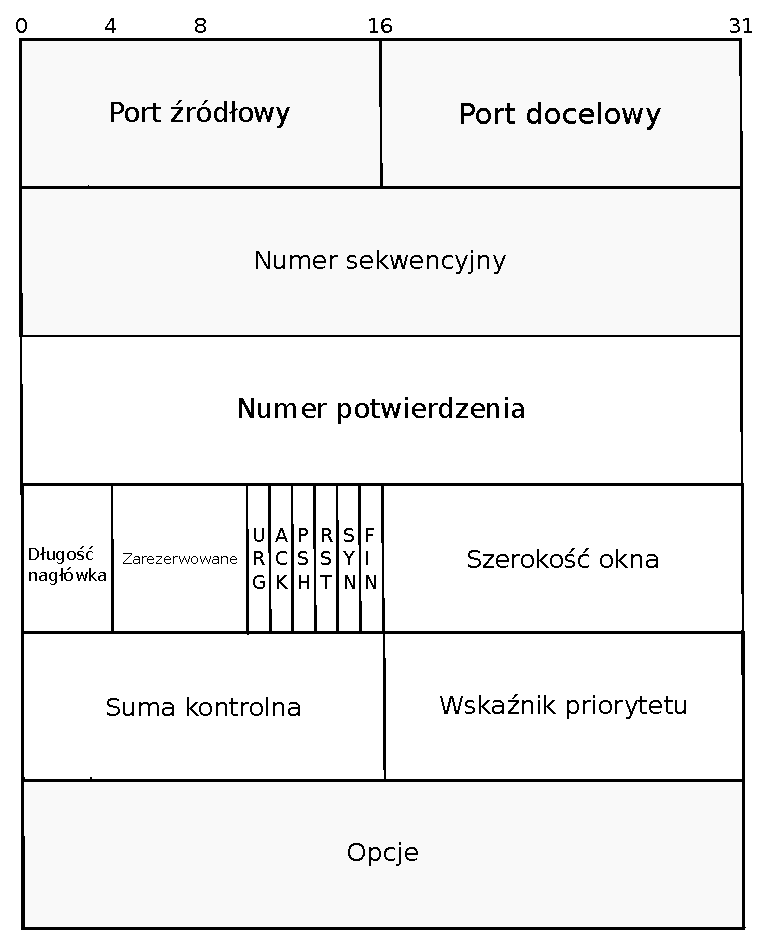
\includegraphics[scale=0.6]{tcp_header}
                \caption{Format nagłówka segmentu protokołu TCP}
                \label{TCPHEADER}
        \end{figure}
        \begin{figure}[h]
                \centering
                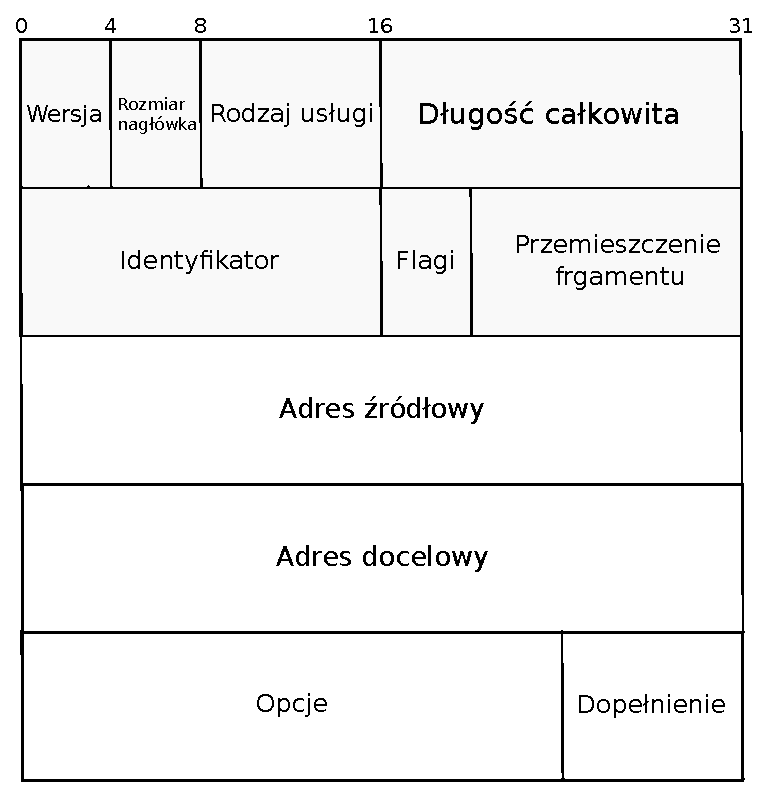
\includegraphics[scale=0.6]{ip_header}
                \caption{Format nagłówka pakietu protokołu IP}
                \label{IPHEADER}
        \end{figure}
        \subsection{Wykorzystanie dopełnienia jednostek danych protokołu}
        Innym sposobem, który można wykorzystać do tworzenia kanałów ukrytych
        jest wykorzystanie pola dopełnienia, o ile takie istnieje.
        Wykorzystanie dopełnienia przez protokół komunikacyjny
        może być konieczne z kilku powodów:
        \begin{itemize}
            \item Niektóre algorytmy kryptograficzne, w~szczególności
        tak zwane szyfry blokowe, operują na stałym z góry określonym fragmencie danych,
        to znaczy bloku. Taki algorytm nie jest w~stanie pracować z danymi, których
        rozmiar nie jest równy rozmiarowi bloku. Jeśli długość
        danych zawartych w~pakiecie nie jest wielokrotnością długości bloku
        algorytmu używanego do szyfrowania, muszą one zostać uzupełnione, aby możliwe
        było zaszyfrowanie całego pakietu. Taka sytuacja występuje w~protokołach,
        które wykorzystują szyfrowanie, na przykład IPSec\cite{IPSECPADDING}.
            \item Dopełnienie pakietu jest konieczne, gdy protokół zakłada, z góry ustaloną długość
        całego pakietu, lub któregoś z pól nagłówka. Takie założenia spotykane są
        w~protokołach, w~których można z dużą dokładnością z góry przewidzieć jaką długość
        będą miały transmitowane dane. W~przypadku, gdy długość danych może oscylować
        wokół przewidzianej wartości, należy założyć długość pakietu (nagłówka)
        nieco większą niż oszacowana. Gdy długość danych do transmisji jest krótsza niż
        założona długość pakietu (nagłówka), konieczne jest zastosowanie dopełnienia.
            \item Niekiedy, dopełnienie stosuje się w~celu dopasowania długości pola nagłówka,
        do długości słowa maszynowego używanego przez dany system komputerowy. Może
        to w~istotny sposób ułatwić implementację sprzętową danego protokołu, lub
        przyspieszyć jego działanie. Ponadto nawet programowe implementacje zyskują
        na szybkości, ponieważ komputery są zoptymalizowane pod względem operowania
        na danych o~długości będącej wielokrotnością długości słowa maszynowego.
        \end{itemize}

        Podobnie jak w~przypadku pól nieużywanych, teoretycznie w specyfikacji
        zapisane jest, jaką wartością powinno odbywać się dopełnianie jednostek danych protokołu.
        Co więcej,
        w~przypadku dopełniania jednostek danych dla algorytmu kryptograficznego, zastosowanie
        nieodpowiedniego dopełnienienia może mieć wpływ na bezpieczeństwo szyfrogramu (złe dopełnienie narażone
        jest na atak "padding oracle attack"). Różnice w~implementacji protokołów
        i~sterowników urządzeń sieciowych, powodują, że dopełnienie można wykorzystać,
        jako miejsce ukrycia danych\cite{PADSTEG}.

        Również tak jak w~przypadku wykorzystania zarezerwowanych pól nagłówka,
        wykrycie tego rodzaju danych ukrytych może zostać sprowadzone do testowania
        zgodności przesyłanych jednostek danych ze specyfikacją protokołu. Wcześniej wspomniane
        wykorzystanie wielu protokołów z różnych warstw sieciowych, pozwala zmniejszyć
        prawdopodobieństwo wykrycia ukrytych wiadomości. Przykład implementacji
        takiego kanału ukrytego przedstawiono w~\cite{PADSTEG}.

        \subsection{Ukrywanie danych w~celowo uszkodzonych jednostkach danych protokołu} \label{USZKODZONEPAKIETY}
        Popularne jest także wykorzystanie mechanizmów zapewniania niezawodności
        transmisji do organizacji kanałów ukrytych. Chodzi tutaj o~mechanizmy
        takie jak odrzucanie i~retransmisja uszkodzonych jednostek danych. Przykładem wykorzystania takich
        mechanizmów jest umyślne tworzenie jednostek danych, w~których suma kontrolna w~nagłówku
        nie zgadza się z sumą kontrolną obliczoną dla treści wiadomości.

        Teoretycznie możliwe są dwa
        sposoby organizacji kanałów ukrytych oparte na tym pomyśle. Pierwszy z nich polega na umieszczeniu
        danych ukrytych w~polu nagłówka, w~którym zwykle znajduje się suma kontrolna,
        jednak nie ma on praktycznego zastosowania, ze względu, na małą przepływność
        kanału ukrytego i~stosunkowo łatwą wykrywalność (transmisja dużej ilości
        danych ukrytych znacząco pogarsza jakość obsługi w~kanale podstawowym).

        Inny pomysł polega
        na umieszczeniu danych ukrytych w~polu danych jednostki danych, i~sfałszowaniu sumy
        kontrolnej. W~takiej sytuacji jednostka danych wygląda na uszkodzoną, w~związku z tym
        dla podsłuchującego i~dla odbiorcy wiadomości podstawowych wydaje się
        ona nie przenosić żadnych użytecznych danych. Odbiorca wiadomości ukrytych,
        widząc, że to właśnie w~takich jednostkach danych znajdują się wiadomości ukryte,
        może je odczytać. Kanały ukryte oparte na takiej zasadzie, są w~stanie
        zapewnić dużą przepływność, należy jednak uważać, aby liczba wprowadzonych
        uszkodzonych jednostek danych mieściła się w~granicach zdrowego rozsądku, zbyt duża
        ich liczba może przyczynić się do wzrostu wykrywalności kanału. Do wad takiego
        rozwiązania należy zaliczyć brak możliwości wykorzystania kanału, jeśli do
        komunikacji pomiędzy nadawcą a~odbiorcą konieczne jest wykorzystanie pośrednika (na przykład routera).
        Jest to spowodowane tym, że zazwyczaj każdy z węzłów pośredniczących w~transmisji
        dokonuje kontroli poprawności jednostki danych (sprawdza sumę kontrolną) i~nie przekazuje
        dalej jednostek uszkodzonych.

        Wykorzystanie celowo uszkodzonych jednostek danych najlepiej sprawdza się w
        sieciach, w~których do naturalnych uszkodzeń jednostek danych, nie związanych z
        istnieniem kanału ukrytego, dochodzi stosunkowo często. W~związku z tym
        świetnie nadają się sieci bezprzewodowe oraz takie, w~których występują
        częste uszkodzenia jednostek danych. Przykład implementacji kanału ukrytego, wykorzystującego
        ukrywanie informacji w~polu danych uszkodzonych jednostek danych, w~sieci Wi-Fi
        został opisany w~\cite{HICCUPS}.

    \section{Poprzez modyfikację właściwości strumienia pakietów} \label{MODYFIKACJASTRUMIENIA}
        \subsection{Poprzez manipulację prędkością transmisji}
        Ten sposób organizacji polega na modulacji prędkości transmisji wiadomości
        pomiędzy nadawcą a~odbiorcą, w~zależności od wiadomości ukrytych, które mają
        być transmitowane. W~przeciwieństwie do poprzednich
        metod, omówionych w rozdziale \ref{MODYFIKACJAPAKIETOW}, tutaj nie następuje
        żadna ingerencja, w~zwartość pola danych ani nagłówka jednostki danych protokołu
        kanału nośnego.

        W~celu organizacji kanału ukrytego wyznaczane są odpowiednie zakresy prędkości, oraz ich
        interpretacja. Odbiorca co ustalony czas, dokonuje próbkowania prędkości
        transmisji. Odczytana wartość jest porównana z umówionymi wcześniej zakresami,
        w~zależności, w~którym z tych zakresów jest ona zawarta, interpretowane jest to
        jako otrzymanie bitu 1, 0 lub brak komunikatu.

        Przepływność takiego kanału ukrytego jest zależna od wybranej przez rozmówców
        częstotliwości próbkowania oraz liczby przedziałów kwantyzacji. Pojawia się
        problem doboru długości przedziałów kwantyzacji, za pomocą których wykonywana
        jest interpretacja wartości
        prędkości chwilowej. Muszą być one na tyle długie, aby uwzględniać naturalnie
        występujące w~sieciach komputerowych opóźnienia oraz przeciążenia, które wpływają
        na chwilową wartość prędkości transmisji. Z drugiej strony, zbyt długie przedziały
        mogą spowodować, że do transmisji danych ukrytych wymagana będzie duża ilość danych
        podstawowych. Ponadto środki przedziałów należy dostosować do natężenia
        napływu wiadomości podstawowych. Możliwe jest wyznaczenie większej ilości
        przedziałów kwantyzacji, co umożliwia transmisję więcej niż jednego bitu w~pojedynczym
        okresie próbkowania.

        Przedstawione problemy powodują, że tego typu kanały muszą być dokładnie
        dobrane pod kątem konkretnej konkretnego środowiska sieciowego, w~którym będą wykorzystywane.
        Zastosowanie takich kanałów w~niestabilnych środowiskach sieciowych (częste zmiany
        opóźnień, lub natężenia napływu danych) jest znacznie utrudnione. Należy jednak
        zauważyć, że po dokładnym skonfigurowaniu oraz przeprowadzeniu dokładnych
        pomiarów opóźnień, kanały ukryte zorganizowane w~ten sposób można z powodzeniem
        stosować, nawet wtedy, gdy do komunikacji konieczne jest korzystanie z węzłów pośrednich.
        Węzły pośrednie, o~ile zachowują się przewidywalnie, nie zmieniają znacznie wcześniej
        zmierzonych wartości opóźnienia oraz prędkości transmisji.

        \subsection{Poprzez manipulację opóźnieniem jednostek danych}
        Sposobem podobnym do poprzedniego jest interpretacja czasu pomiędzy odebraniem kolejnych jednostek danych,
        jako fragmenty pochodzące z danych ukrytych\cite{IPDELAYCHANNEL}. Ten sposób nie wymaga jednak próbkowania,
        ponieważ czas pomiędzy odebraniem dwóch kolejnych jednostek danych
        może być precyzyjnie obliczony. Nadal jednak potrzebna
        jest kwantyzacja, ze względu na wpływ warunków zewnętrznych, takich jak przeciążenia,
        na opóźnienie jednostek danych. Nadawca umyślnie wydłuża lub skraca czas pomiędzy
        wysłaniem kolejnych jednostek danych, w~zależności od fragmentu danych ukrytych,
        które chce przetransmitować. Odbiorca po odebraniu jednostki danych oblicza czas jaki
        upłynął od odebrania poprzedniego jednostki danych, następnie
        interpretuje opóźnienie jako fragment wiadomości ukrytej korzystając z
        przedziałów kwantyzacji.

        Przepływność tak uzyskanego kanału zależy od długości i~ilości wybranych
        przedziałów kwantyzacji. Ma on wiele cech wspólnych z~wcześniej przedstawionym
        kanałem. Podobnie jak w~poprzednim przypadku, wyznaczenie długości
        przedziałów kwantyzacji powinno być poprzedzone zbadaniem opóźnień występujących
        naturalnie w~środowisku sieciowym, ponieważ nakładają się one na opóźniania
        wprowadzone przez nadawcę. W~związku z tym taki kanał ukryty również wrażliwy jest
        na nagłe zmiany charakterystyk pracy sieci komputerowej, jednak w~mniejszym
        stopniu niż kanał oparty na modulacji prędkości transmisji. Równie dobrze
        nadaje się on do komunikacji, gdy pomiędzy odbiorcą a~nadawcą znajdują się
        węzły pośredniczące.

        Zaletą obu przedstawionych w~tej sekcji protokołów komunikacyjnych,
        jest możliwość wykorzystania szerokiego zestawu protokołów jako
        źródeł wiadomości podstawowych. Przedstawione techniki są ogólne i
        nie stawiają żadnych wymagań protokołowi, który zostanie wykorzystany jako
        nośnik (brak wymagań co do określonych pól nagłówka, oraz co do typu transportowanych danych).
        W~związku z tym, jako źródło wiadomości podstawowych może być wykorzystana
        praktycznie każdy aplikacja sieciowa, pod warunkiem odpowiedniego skonfigurowania
        protokołu kanału ukrytego.


    \section{Podejścia hybrydowe}
        \subsection{Ukrywanie danych w~pakietach protokołów strumieniowej transmisji danych}
        W~celu połączenia zalet podejść przedstawionych w~sekcjach
        \ref{MODYFIKACJAPAKIETOW} i~\ref{MODYFIKACJASTRUMIENIA}, oraz wyeliminowania
        ich wad, stworzono kanały steganograficzne, wykorzystujące jednocześnie obie te
        techniki. Takie kanały modyfikują jednocześnie pojedyncze jednostki danych protokołu,
        jak i~właściwości strumienia jednostek danych. Dzięki temu, można przesyłać ukryte wiadomości,
        nawet do innych sieci komputerowych, z wykorzystaniem pośrednich węzłów sieciowych,
        jednocześnie eliminując dużą zależność protokołu kanału ukrytego od warunków
        panujących w~środowisku sieciowym. Ceną, którą należy zapłacić za kanał
        ukryty tej klasy, jest niewielka liczba protokołów, które można wykorzystać
        jako kanał podstawowy. Najczęściej wykorzystywaną klasą protokołów są
        protokoły strumieniowej transmisji danych, wykorzystywane między innymi
        w~aplikacjach VOiP, lub strumieniujących multimedia (muzyka, filmy).

        W~pracy \cite{VOIPSTEGANOGRAPHY} w~celu organizacji kanału ukrytego wykorzystany
        jest protokół RTP (\emph{Real-Time Transfer Protocol}), jako przykład aplikacji
        wykorzystującej ten protokół wybrano aplikację typu VOiP. W~tego typu aplikacjach,
        jeśli odbiorca odbierze pakiet, który jest znacznie opóźniony w~stosunku
        do innych pakietów, uznaje się, że informacje w~nim zawarte są bezwartościowe,
        ponieważ jest za późno, aby użyć je do procedury rekonstrukcji głosu.
        Zastosowane przez autorów podejście opiera się na celowym opóźnianiu pakietów
        zawierających dane ukryte, zapisane w~polu danych pakietu.
        Odbiorca wiadomości podstawowych odbierając pakiet
        opóźniony, odrzuca go, jednak odbiorca wiadomości ukrytych wiedząc, że to właśnie
        w~nim znajduje się ukryta wiadomość, może ją odczytać.

        Pakiet zostaje rozpoznany jako opóźniony, nie tylko ze względu na celowe
        oczekiwanie z~jego wysłaniem przez nadawcę, ale również ze względu
        na umieszczenie sfałszowanego czasu wysłania pakietu w~odpowiednim
        polu nagłówka (pole Timestamp, rysunek \ref{RTPHEADER}). Dzięki temu kanał staje się mniej zależny
        od warunków transmisji i~opóźnienia naturalnie występującego w~sieci komputerowej.

        W~celu realizacji kanału ukrytego modyfikowane są zarówno pola pakietów (pole danych,
        pole nagłówka z czasem nadania), jak i~właściwości strumienia pakietów (opóźnienie).
        Zgodnie z~tym, co wspomniano wcześniej, pozwala to na połączenie zalet obu opisywanych
        wcześniej sposobów organizacji kanałów ukrytych. Ponadto użycie pola danych
        do transmisji danych ukrytych, pozwala na stworzenie kanału ukrytego o
        większej przepływności w stosunku do sposobów organizacji ukrytych kanałów
        przedstawionych w rozdziałach \ref{MODYFIKACJAPAKIETOW} i \ref{MODYFIKACJASTRUMIENIA}.
        Podobnie jak w~przypadku metody omawianej w~sekcji
        \ref{USZKODZONEPAKIETY}, tak i~tutaj ilość pakietów, które zostaną opóźnione
        nie może być zbyt duża, ponieważ może to skutkować znaczącym pogorszeniem
        jakości usługi i~ułatwić wykrycie kanału ukrytego.

        \begin{figure}[h]
                \centering
                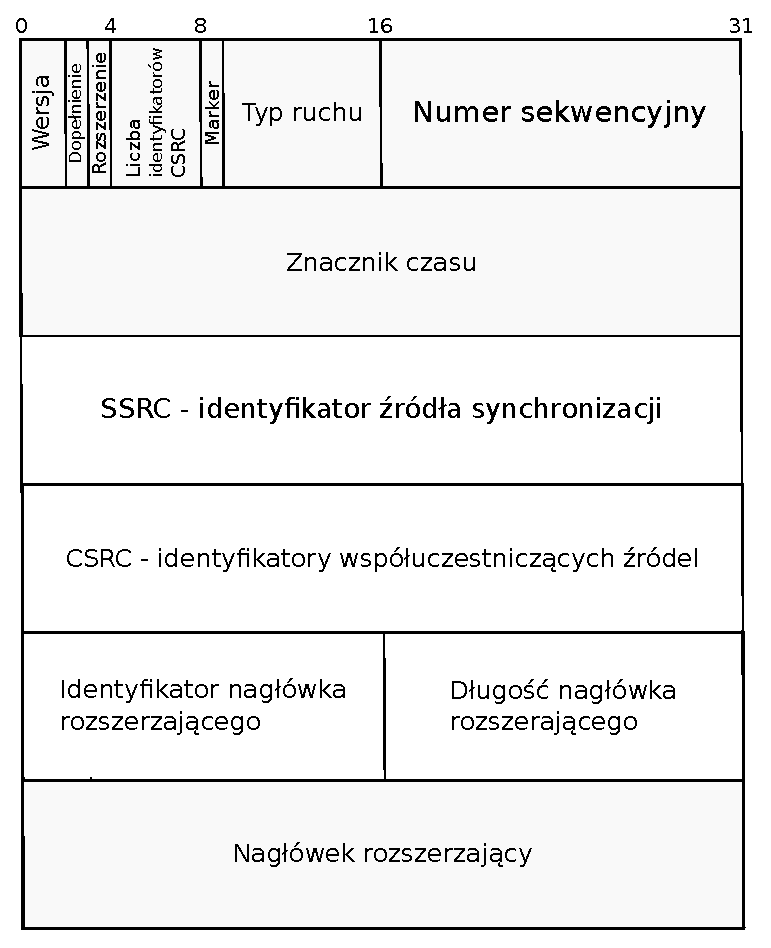
\includegraphics[scale=0.8]{rtp_header}
                \caption{Format nagłówka pakietu protokołu RTP}
                \label{RTPHEADER}
        \end{figure}

\chapter{Projekt protokołu kanału ukrytego}
    \section{Słownik używanych pojęć} \label{DICT}
    \begin{itemize}
        \item \emph{Kanał podstawowy (nośnik)} - kanał, w~którym zarówno fakt komunikacji,
            jak również treść przesyłanych wiadomości, jest widoczna dla osób postronnych,
            jednostki danych protokołu użytego do jego realizacji są modyfikowane przez
            protokół kanału ukrytego;

        \item \emph{Wiadomość podstawowa (\(W_P\))} - wiadomość transmitowana kanałem
            podstawowym;

        \item \emph{Kolejka wiadomości podstawowych ( \( K_{WP} \) )} - kolejka,
                wykorzystywana w algorytmie kanału ukrytego, w
                której przechowywane są, ze względu na brak możliwości natychmiastowej
                transmisji, wiadomości podstawowe, jednostką pojemności kolejki
                wiadomości podstawowych jest bajt;

        \item \emph{Kanał ukryty} - kanał umożliwiający transmisję wiadomości w~taki sposób,
            aby osoba postronna obserwująca kanał transmisyjny nie była świadoma
            nie tylko treści wiadomości, ale również faktu, że transmisja wiadomości ma miejsce;

        \item \emph{Wiadomość ukryta (\(W_U\))} - wiadomość transmitowana kanałem ukrytym;

        \item \emph{Kolejka wiadomości ukrytych ( \( K_{WU} \) )} - kolejka,
                wykorzystywana w algorytmie kanału ukrytego, w~której
                przechowywane są, ze względu na brak możliwości natychmiastowej
                transmisji, wiadomości ukryte, jednostką pojemności kolejki
                wiadomości podstawowych jest bit;

        \item \emph{Segment wiadomości ukrytej (\(S_{WU}\))} - fragment,
            wiadomości ukrytej, który jest transmitowany (w sposób ukryty) w~jednej
            jednostce danych protokołu kanału podstawowego;

        \item \emph{Długość segmentu wiadomości ukrytej (\( L_{SWU} \))} - liczba
                pozycji binarnych zawartych w~jednym segmencie danych ukrytych;

        \item \emph{Wartość segmentu wiadomości ukrytej (\( V_{SWU} \))} - wartość
            liczbowa segmentu wiadomości ukrytej potraktowanego, jako liczba binarna,
            na przykład dla segmentu wiadomości ukrytej o~treści 11010011:
            \( V_{SWU}(11010011) = 211 \);

       \item \emph{Maksymalna wartość segmentu wiadomości ukrytej (\( Max_{V_{SWU}} \))} -
           maksymalna wartość, segmentu wiadomości ukrytej przy
           założonej wartości długości segmentu wiadomości ukrytej, czyli wartość
           segmentu wiadomości ukrytej, w~którym wszystkie bity mają wartość 1,
           na przykład dla \( L_{SWU} = 8 \), segment o~wartości maksymalnej to
           \( 11111111 \), a~jego wartość to: \( Max_{V_{SWU}} = 255 \);

       \item \emph{Fragmentacja wiadomości podstawowych} -
           procedura podziału jednej wiadomości podstawowej na
           kilka mniejszych, w celu transmisji kilku segmentów wiadomości ukrytej

       \item \emph{Agregacja wiadomości podstawowych} - procedura syntezy większej wiadomości
           z~kilku małych, w celu transmisji segmentu wiadomości ukrytej, lub transmisji
           pakietu bez danych ukrytych

       \item \emph{Błąd komunikacji} - odebranie przez odbiorcę
           jednostki danych zawierającej inną treść niż została w~niej
           umieszczona przez nadawcę, wyróżniamy błędy podstawieniowe, które
           zmieniają wartość pojedynczych bitów wiadomości, lub błędy wtrąceniowe,
           które powodują utratę, lub odbiór większej ilości bitów niż wysłał nadawca;

    \end{itemize}

    \section{Założenia i~ograniczenia projektowe}
    Na potrzeby protokołu kanału ukrytego i~jego badań przyjęto następujące założenia
    dotyczące modelu systemu komunikacyjnego, złożonego z~kanału komunikacyjnego
    podstawowego i~wbudowanego kanału komunikacyjnego ukrytego:
    \begin{enumerate}
        \item \emph{Pojemność kolejki wiadomości ukrytych i~podstawowych jest nieograniczona} -
            jak zostanie omówione w~następnym rozdziale, działanie protokołu
            kanału ukrytego wymaga kolejkowania zarówno wiadomości podstawowych
            jak i~ukrytych. W~obecnej wersji protokół kanału ukrytego nie wspiera
            żadnego mechanizmu radzenia sobie z przeciążeniami, w~związku z tym
            dla ułatwienia prowadzenia badań, założono nieskończoną pojemność obu kolejek.

        \item \emph{Wiadomość (zarówno podstawową jak i~ukrytą) traktujemy, jako odebraną,
            gdy wszystkie jej segmenty zostaną odebrane przez odbiornik} - jak powiedziano
            wcześniej, wiadomości ukryte mogą składać się z więcej niż jednego segmentu,
            natomiast jak zostanie powiedziane, wiadomości podstawowe mogą być fragmentowane
            w~celu transmisji pakietów z ukrytymi wiadomościami. Aby umożliwić
            obliczanie opóźnień zarówno wiadomości podstawowych jak i~ukrytych,
            zakłada się, że opóźnienie to czas pomiędzy napłynięciem wiadomości,
            a~odebraniem ostatniego jej segmentu.

        \item \emph{Komunikacja pomiędzy odbiorcą a~nadawcą odbywa się bez błędów komunikacji} -
            jak wspomniano wcześniej, protokół UDP jest protokołem zawodnym.
            Zaprojektowany protokół kanału ukrytego również nie zapewnia mechanizmów niezawodnej
            transmisji danych. Aby nie komplikować metodologii
            obliczania opóźnień poszczególnych wiadomości, związanych z utratą
            pakietów je transportujących, założono, że w~trakcie transmisji nie
            występują żadne błędy, zarówno podstawieniowe jak i~wtrąceniowe.

        \item \emph{Długość wiadomości ukrytej jest wielokrotnością długości segmentu
            wiadomości ukrytej (\(L_{SWU}\))} - długość każdego odebranego przez odbiorcę pakietu,
            jest przez niego interpretowana jako wartość segmentu danych ukrytych o~określonej
            długości. Powoduje to konieczność zapewnienia, że wszystkie segmenty
            wiadomości ukrytej są tej samej długości i~są w~pełni wypełnione, co czasami
            wymaga zastosowania dopełnienia. Przyjęcie tego założenie upraszcza protokół
            kanału ukrytego, ponieważ odpowiedzialność za dopełnienie wiadomości ukrytych
            spada na użytkownika kanału.
    \end{enumerate}

    \section{Opis otoczenia działania protokołu}
    W~proponowanym protokole kanału ukrytego długość pola danych pakietu protokołu UDP
    jest równa:
    \begin{itemize}
        \item wartości kolejnego segmentu kolejnej wiadomości ukrytej, w przypadku
            gdy wiadomość podstawowa jest modyfikowana wiadomością ukrytą, lub
        \item jest równa sumie długości pól danych wiadomości podstawowych, w przypadku
            gdy wiadomość (ciąg wiadomości) podstawowa nie jest modyfikowana wiadomościami
            ukrytymi
    \end{itemize}
    Kanał ukryty przeznaczony jest do komunikacji typu punkt-punkt i może być
    wykorzystywany zarówno do komunikacji w połączeniach sieciowych z węzłami
    pośrednimi i bez węzłów pośrednich. Protokół UDP jest protokołem datagramowym, co
    oznacza, że każdy pakiet jest traktowany jako całość i nie może
    być zarówno dzielony jak i agregowany z innymi.

    Z uwagi na to, że pakiety modyfikowane przez protokół kanału ukrytego, to pakiety UDP,
    w~dalszej części pracy zakłada się, że protokół warstwy aplikacji kanału podstawowego jest oparty o~UDP.
    Porady dotyczące wyboru konkretnego protokołu warstwy aplikacji dla
    kanału podstawowego są przedstawione w~sekcji \ref{SUGESTIEPARAMETROW}. Sam protokół kanału
    ukrytego, może działać z~różnymi protokołami warstwy aplikacji kanału podstawowego.
    Jedynym wymaganiem co do protokołu warstwy aplikacji kanału podstawowego
    jest wykorzystanie protokołu UDP do transmisji danych. Podobnie wygląda sytuacja,
    jeśli chodzi o~protokoły warstw niższych niż warstwa transportowa. Protokół kanału
    ukrytego może funkcjonować we wszystkich sieciach obsługujących protokół UDP.

    \section{Model protokołu kanału ukrytego}

    Model kanału ukrytego został przedstawiony na rysunku \ref{HIDDENCHANNELMODEL}.
    Oznaczone na nim zostały:
    \begin{itemize}
        \item Źródło danych podstawowych -
    charakteryzowane jest dwoma parametrami: średnim natężeniem, to jest średnią liczbą
    wiadomości napływających w jednostce czasu, oraz średnią długością wiadomości (w~bajtach).
        \item Kolejka wiadomości podstawowych - pionowa kolejka znajdująca się pod
    źródłem wiadomości podstawowych, zawiera w sobie wiadomości podstawowe,
    każda z wiadomości opisana jest przez długość wiadomości podstawowej.
        \item Kanał podstawowy - charakteryzowany jest
    poprzez jego pojemność, wyrażona jest ona w~bitach na sekundę. Ogranicza ona
    maksymalną ilość danych, możliwych do przesłania kanałem w~jednostce czasu i
    w~rezultacie może wpływać na opóźnienie wiadomości podstawowych i~ukrytych.
        \item Źródło wiadomości ukrytych - charakteryzowane jest rozkładami:
            \begin{itemize}
                \item natężenia napływu wiadomości ukrytych,
                \item długości wiadomości (w segmentach na wiadomość),
                \item wartości segmentów
            \end{itemize}
        \item Kolejka wiadomości ukrytych - znajduje się na prawo od źródła wiadomości ukrytych.
            Zawiera dwie wiadomości ukryte, każda z nich jest opisana jest długością wiadomości.
        \item Kolejka segmentów wiadomości ukrytych - znajduje się na prawo od kolejki
            wiadomości ukrytych, zawiera segmenty wiadomości ukrytych, powstałe w procesie
            segmentacji wiadomości ukrytych. Każdy segment jest opisany przez wartość segmentu.
    \end{itemize}

    \begin{figure}[h]
            \centering
            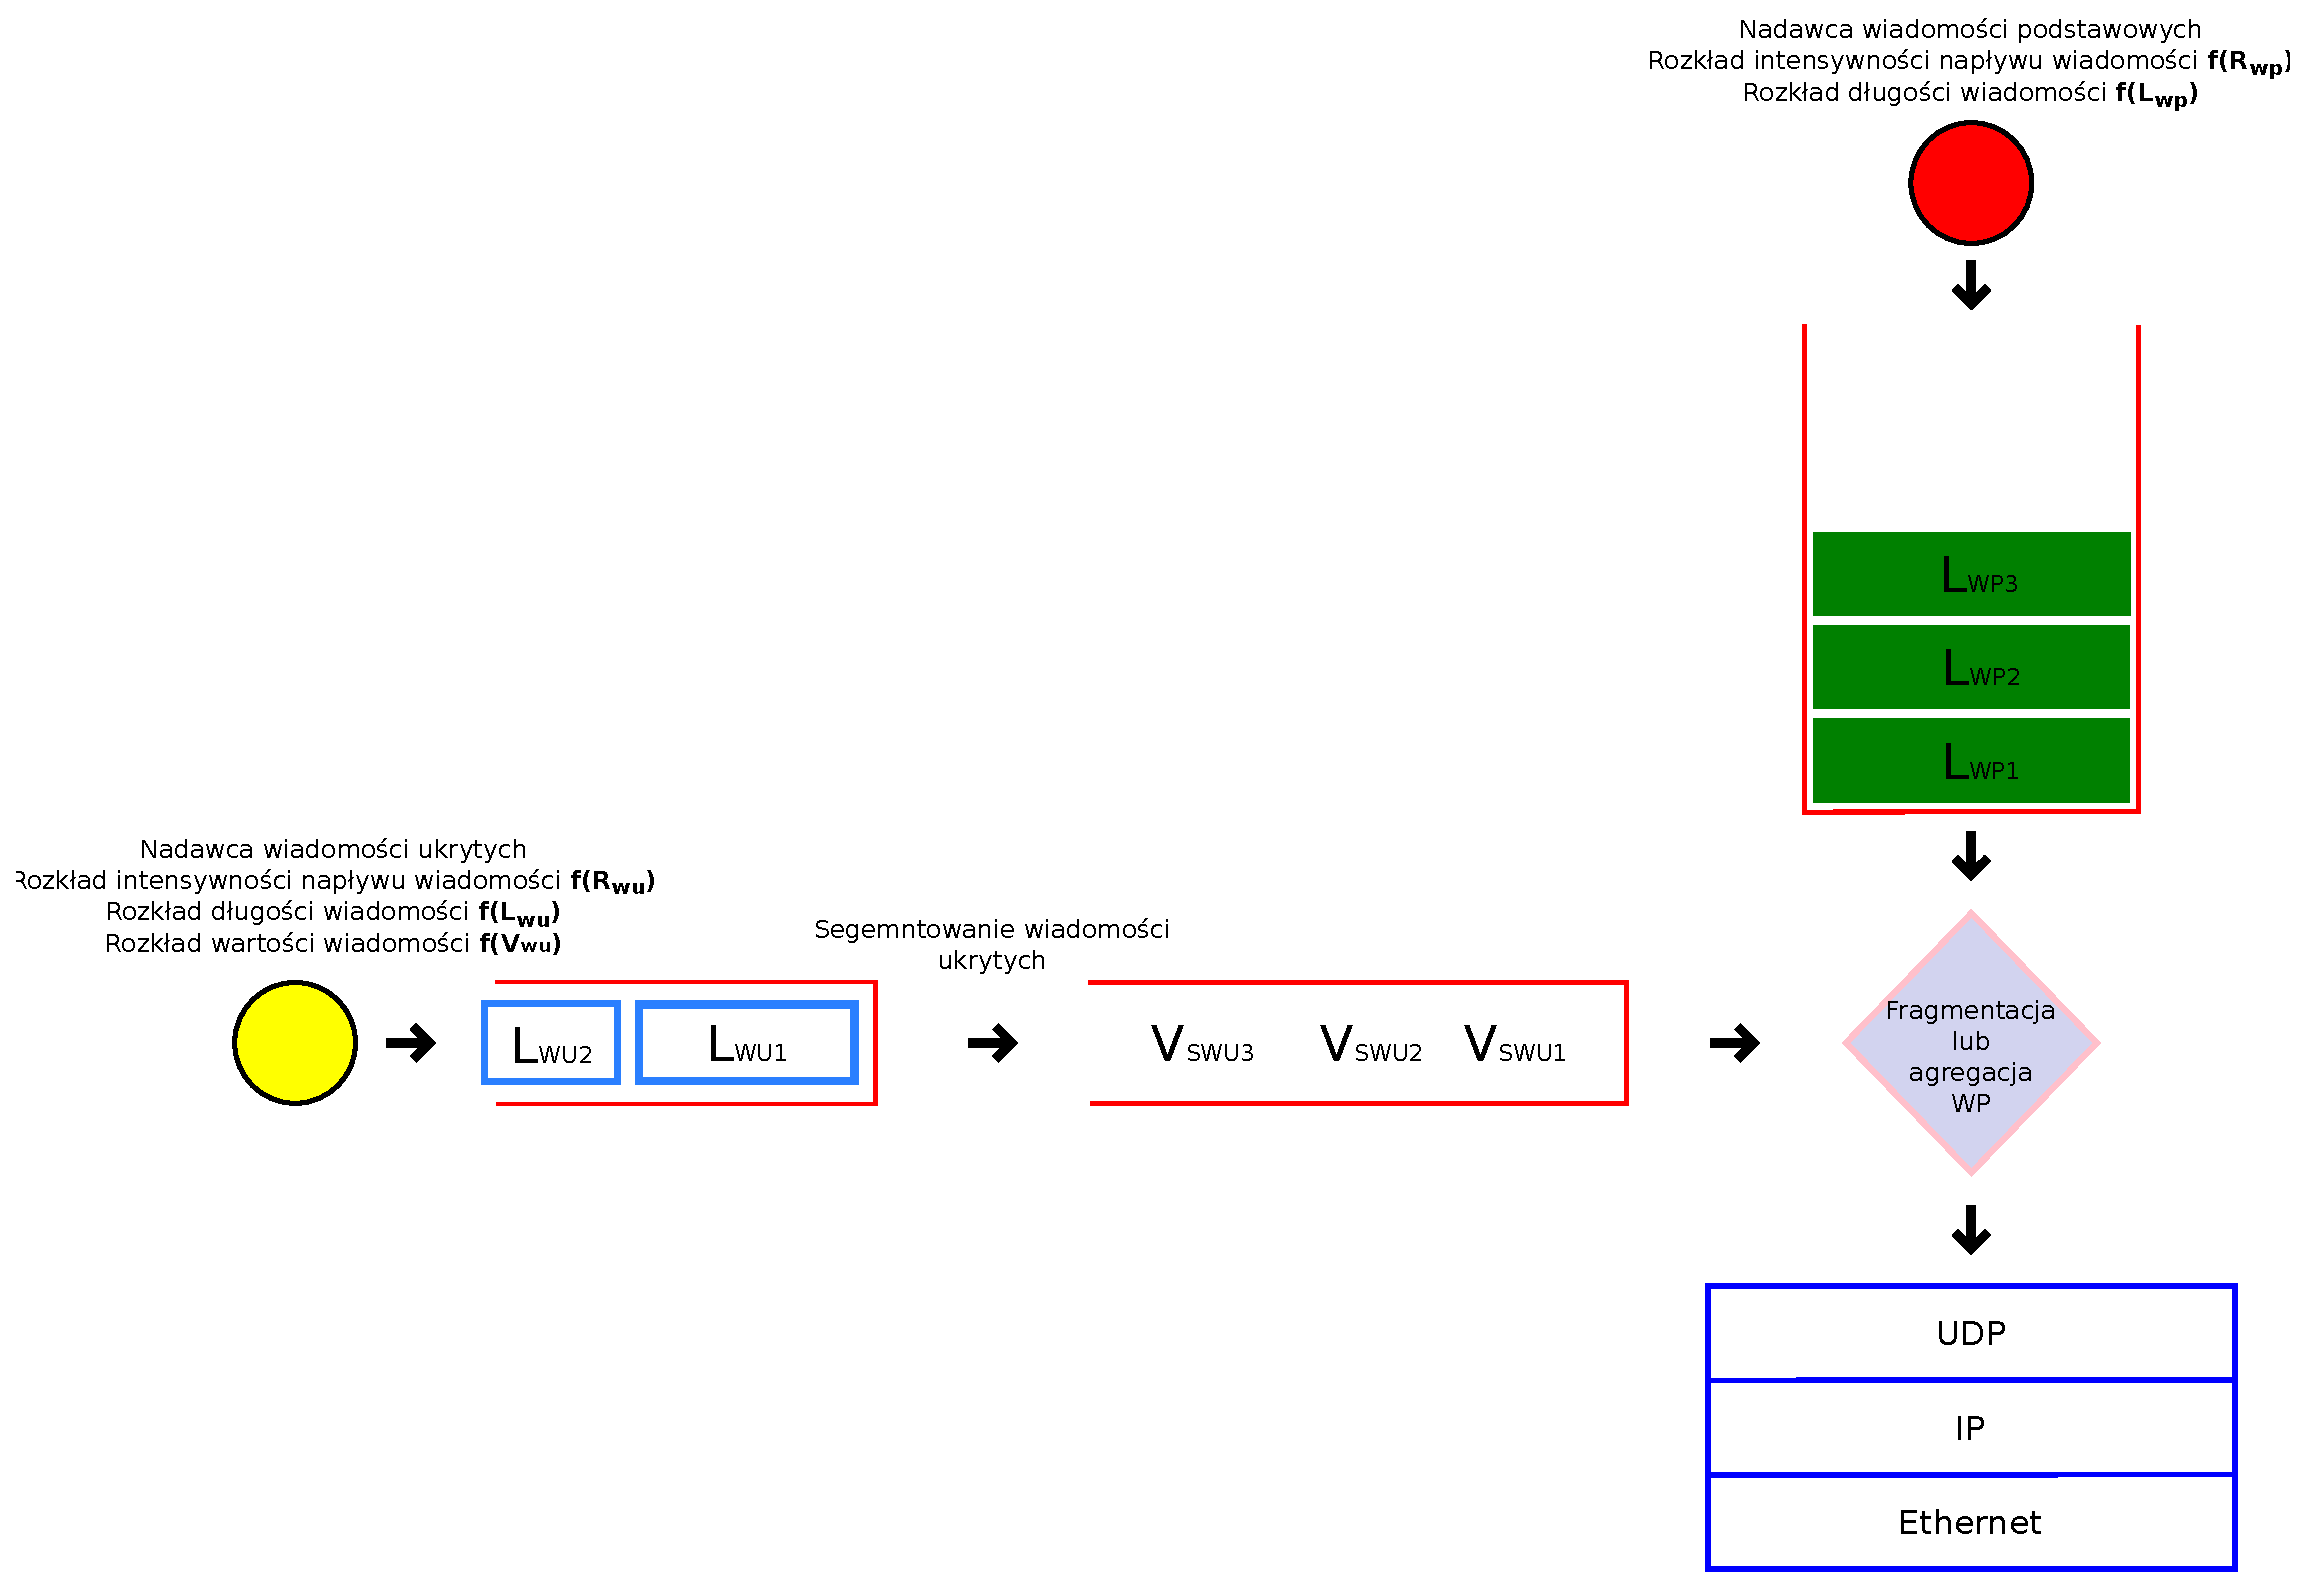
\includegraphics[scale=0.45]{hidden_channel_model}
            \caption{Model kanału ukrytego}
            \label{HIDDENCHANNELMODEL}
    \end{figure}

    \section{Opis działania protokołu kanału ukrytego} \label{CHANNELDESCRIPTION}
    Protokół kanału ukrytego konfigurowany jest przy pomocy pojedynczego parametru -
    długość segmentu wiadomości ukrytej \( L_{SWU} \), którego jednostką są bity.
    Parametr ten określa, na jakiej długości segmenty zostanie podzielona wiadomość
    ukryta. Musi on zostać uzgodniony przez komunikujące się za pomocą kanału
    ukrytego strony, przed rozpoczęciem komunikacji. Schemat podziału wiadomości
    podstawowych jest przedstawiony na rysunku \ref{SEGMENTATION}, gdzie za długość
    segmentu wiadomości ukrytej przyjęte zostało 10 bitów.
    Ponadto na schemacie kolorem czerwonym zaznaczono dopełnienie, dzięki któremu
    każdy z segmentów ma taką samą długość. W~przedstawionym przykładzie wiadomość
    jest tekstem, w~związku z czym, jako krok pośredni, kody ASCII liter, z których
    jest złożona zostają zamienione na ciągi bitów. Jak wcześniej wspomniano, protokół
    kanału ukrytego nie dopełnia segmentów, jest to zadanie użytkownika protokołu.
        \begin{figure}[h]
                \centering
                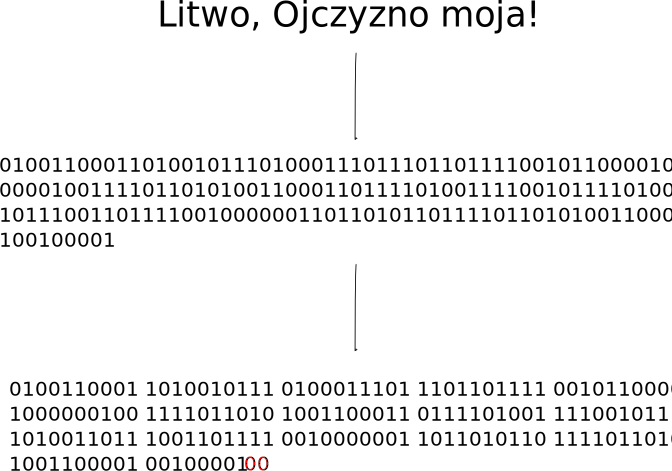
\includegraphics[scale=0.8]{podzial_na_segmenty}
                \caption{Kodowanie i  podział wiadomości ukrytej na 10-elementowe binarne segmenty}
                \label{SEGMENTATION}
        \end{figure}

    Po podziale, segmenty wiadomości ukrytej zostają umieszczone w~kolejce segmentów wiadomości
    ukrytych. Kolejka ta, jest kolejką typu FIFO (First In, First Out).
    Do utworzenia kolejnego pakietu przenoszącego pierwszy segment z kolejki
    segmentów wiadomości ukrytych niezbędny jest ciąg wiadomości podstawowych,
    których suma długości (w bajtach) jest nie mniejsza niż wartość tego segmentu wiadomości ukrytych.
    Dane służące do zbudowania
    jednego pakietu przenoszącego segment wiadomości ukrytej, mogą pochodzić z wielu wiadomości
    podstawowych, jak również jedna wiadomość podstawowa może zostać użyta do zbudowania
    wielu \emph{pakietów przenoszących segmenty wiadomości ukrytych}. Jeśli suma długości wiadomości
    podstawowych w~kolejce jest większa, niż potrzebna do transmisji danych ukrytych, niewykorzystane
    wiadomości podstawowe pozostają w~kolejce, aby mogły być wykorzystane do transmisji
    kolejnego segmentu wiadomości ukrytej.
    W~przypadku, gdy suma długości wiadomości znajdujących się kolejce jest mniejsza
    niż wartość segmentu wiadomości ukrytej, pozostaje on w~kolejce i oczekuje
    na zgromadzenie większej ilości wiadomości podstawowych.

    W~sytuacji, gdy napłynie wiadomość podstawowa, jest ona dodawana do kolejki
    wiadomości podstawowych, która również jest kolejką typu FIFO.
    Podobnie jak w~przypadku napłynięcia wiadomości ukrytej, sprawdzana jest możliwość
    transmisji pakietu z danymi ukrytymi. Może się ona odbyć, gdy w~kolejce wiadomości
    ukrytych oczekuje segment wiadomości ukrytej, a~suma długości wiadomości w~kolejce wiadomości
    podstawowych (licząc nowo dodaną wiadomość podstawową), jest równa lub większa
    od wartości segmentu wiadomości ukrytej. Jeśli ten warunek nie jest spełniony, wiadomości podstawowa
    pozostaje w~kolejce i~oczekuje na wiadomość ukrytą.

    Kolejkowanie wiadomości podstawowych, w~przypadku znacznie intensywniejszego
    napływu wiadomości podstawowych niż wiadomości ukrytych, może prowadzić do
    występowania dużych opóźnień wiadomości podstawowych. W~skrajnym przypadku,
    gdy napływ wiadomości ukrytych ustaje całkowicie, komunikacja w kanale podstawowym staje się niemożliwa.
    Z powodu konstrukcji protokołu kanału
    ukrytego, wysyłanie wiadomości podstawowych, bez danych ukrytych i bez odpowiedniego ich oznaczenia jest niemożliwe.
    Takie wiadomości mogłyby zostać błędnie zinterpretowane przez odbiornik wiadomości
    ukrytych, jako fragmenty wiadomości ukrytych. Konieczne jest znalezienie mechanizmu,
    który: (A) pozwala na funkcjonowanie kanału podstawowego i~transmisję wiadomości
    podstawowych, nawet wtedy, gdy napływ wiadomości ukrytych ustanie, oraz (B)
    pozwoli odpowiednio oznaczyć pakiety nie zawierające segmentu wiadomości ukrytej, tak aby ich długość
    nie była interpretowana przez odbiorcę wiadomości ukrytych, jako ich fragment.

    Dla przedstawianego protokołu kanału ukrytego, proponowane jest następujące
    rozwiązanie. Każdy pakiet UDP wygenerowany przez protokół kanału ukrytego,
    niesie informację o~wartości dokładnie jednego segmentu wiadomości ukrytej.
    Z przedstawionego wcześniej mechanizmu
    działania kanału ukrytego, wynika, że dla danej wartości parametru \( L_{SWU} \),
    nigdy nie wygeneruje on pakietu UDP o~długości większej, niż odpowiadająca parametrowi
    \( L_{SWU} \) maksymalna wartość segmentu wiadomości ukrytej \( Max_{V_{SWU}} \).
    Dla przypomnienia jest ona obliczana ze wzoru:
    \begin{math}
        Max_{V_{SWU}} = 2^{L_{SWU}} - 1
    \end{math}.
    Do przesyłania pakietów nie zawierających danych ukrytych, proponowane jest
    wykorzystanie pakietów o~długości większej niż maksymalna wartość segmentu
    wiadomości ukrytej, przy zadanej konfiguracji protokołu kanału ukrytego. W~momencie,
    gdy po napłynięciu wiadomości podstawowej, zostanie stwierdzony brak wiadomości
    ukrytych oczekujących na transmisję, sprawdzane jest, czy suma długości wiadomości
    w~kolejce wiadomości podstawowych (wraz z nowo przybyłą wiadomością), jest
    większa niż \( Max_{V_{SWU}} \), jeśli tak, to cała zawartość kolejki wiadomości
    podstawowych jest wysyłana jednym pakietem UDP. Odbiorca, widząc pakiet o~długości
    większej niż maksymalna wartość segmentu wiadomości ukrytej, wie, że nie powinien
    jego długości interpretować jako fragmentu danych ukrytych. W~dalszej części
    pracy, pakiety wygenerowane w~ten sposób nazywane będą
    \emph{pakietami nieprzenoszącymi segmentów wiadomości ukrytych}.

    Na rysunku \ref{COMMUNICATION} przedstawiono przebieg przykładowej komunikacji
    za pomocą prezentowanego kanału ukrytego, przy założeniu, że \( L_{SWU} = 5 \) bitów.
    Przy takiej konfiguracji:
    \begin{math}
        Max_{V_{SWU}} = 2^{L_{SWU}} - 1 = 2^5 - 1 = 31
    \end{math}.
    Na schemacie można zaobserwować, że dwa pierwsze pakiety wysłane przez nadawcę
    są pakietami zawierającymi dane ukryte, w~związku z czym odbiorca interpretuje
    ich długość jako wartość segmentów wiadomości ukrytych. Ostatni wysłany pakiet
    jest pakietem nieprzenoszącym segmentu wiadomości ukrytej.
    Zgodnie ze wcześniejszym opisem, ponieważ jego długość jest większa niż maksymalna
    wartość segmentu danych ukrytych, odbiorca nie odczytuje z takiego pakietu
    segmentu wiadomości ukrytej.
        \begin{figure}[h]
                \centering
                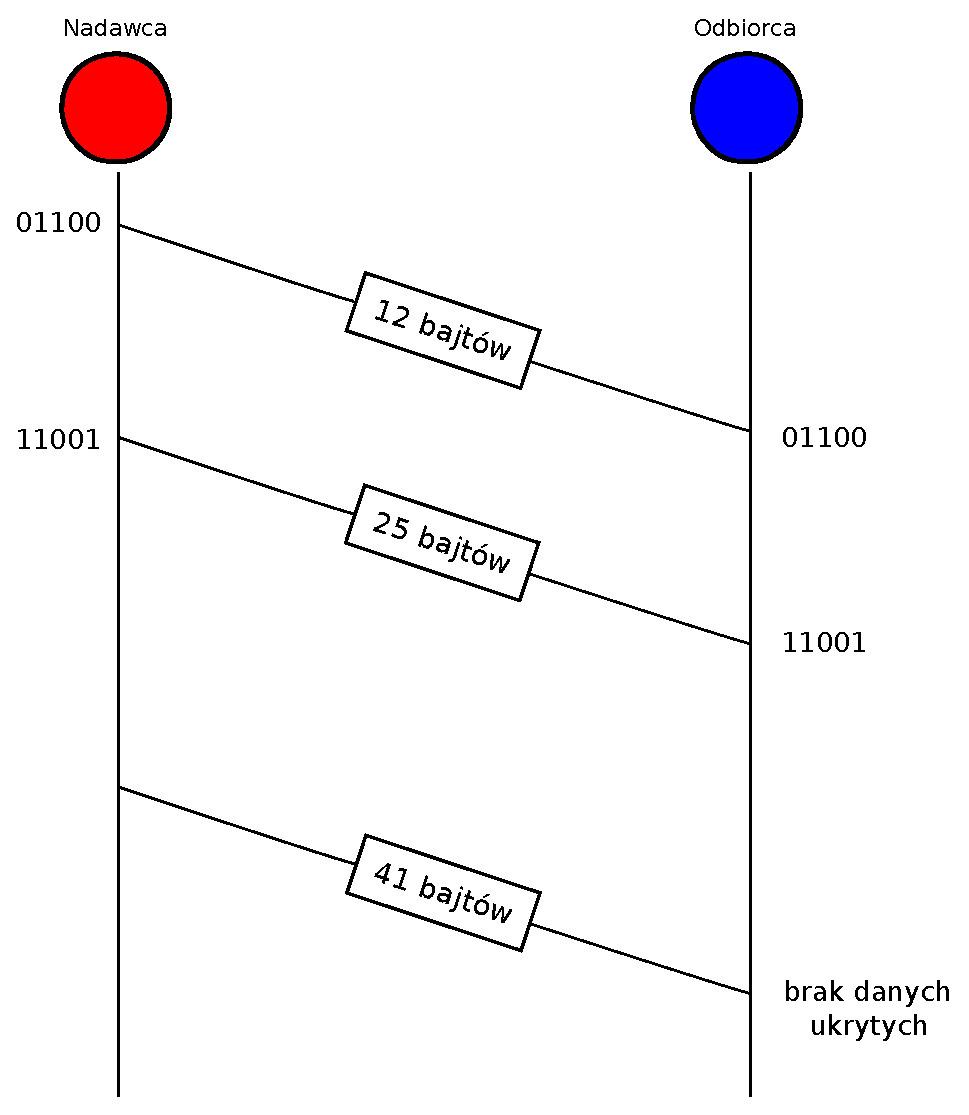
\includegraphics[scale=0.85]{komunikacja_kanalem_ukrytym_gotowa}
                \caption{Przykładowa komunikacja kanałem ukrytym}
                \label{COMMUNICATION}
        \end{figure}

    Schemat algorytmu działania protokołu kanału ukrytego, opisany w~tej sekcji,
    przedstawia rysunek \ref{CHANNELALGORITHM}.

        \begin{figure}[h]
                \centering
                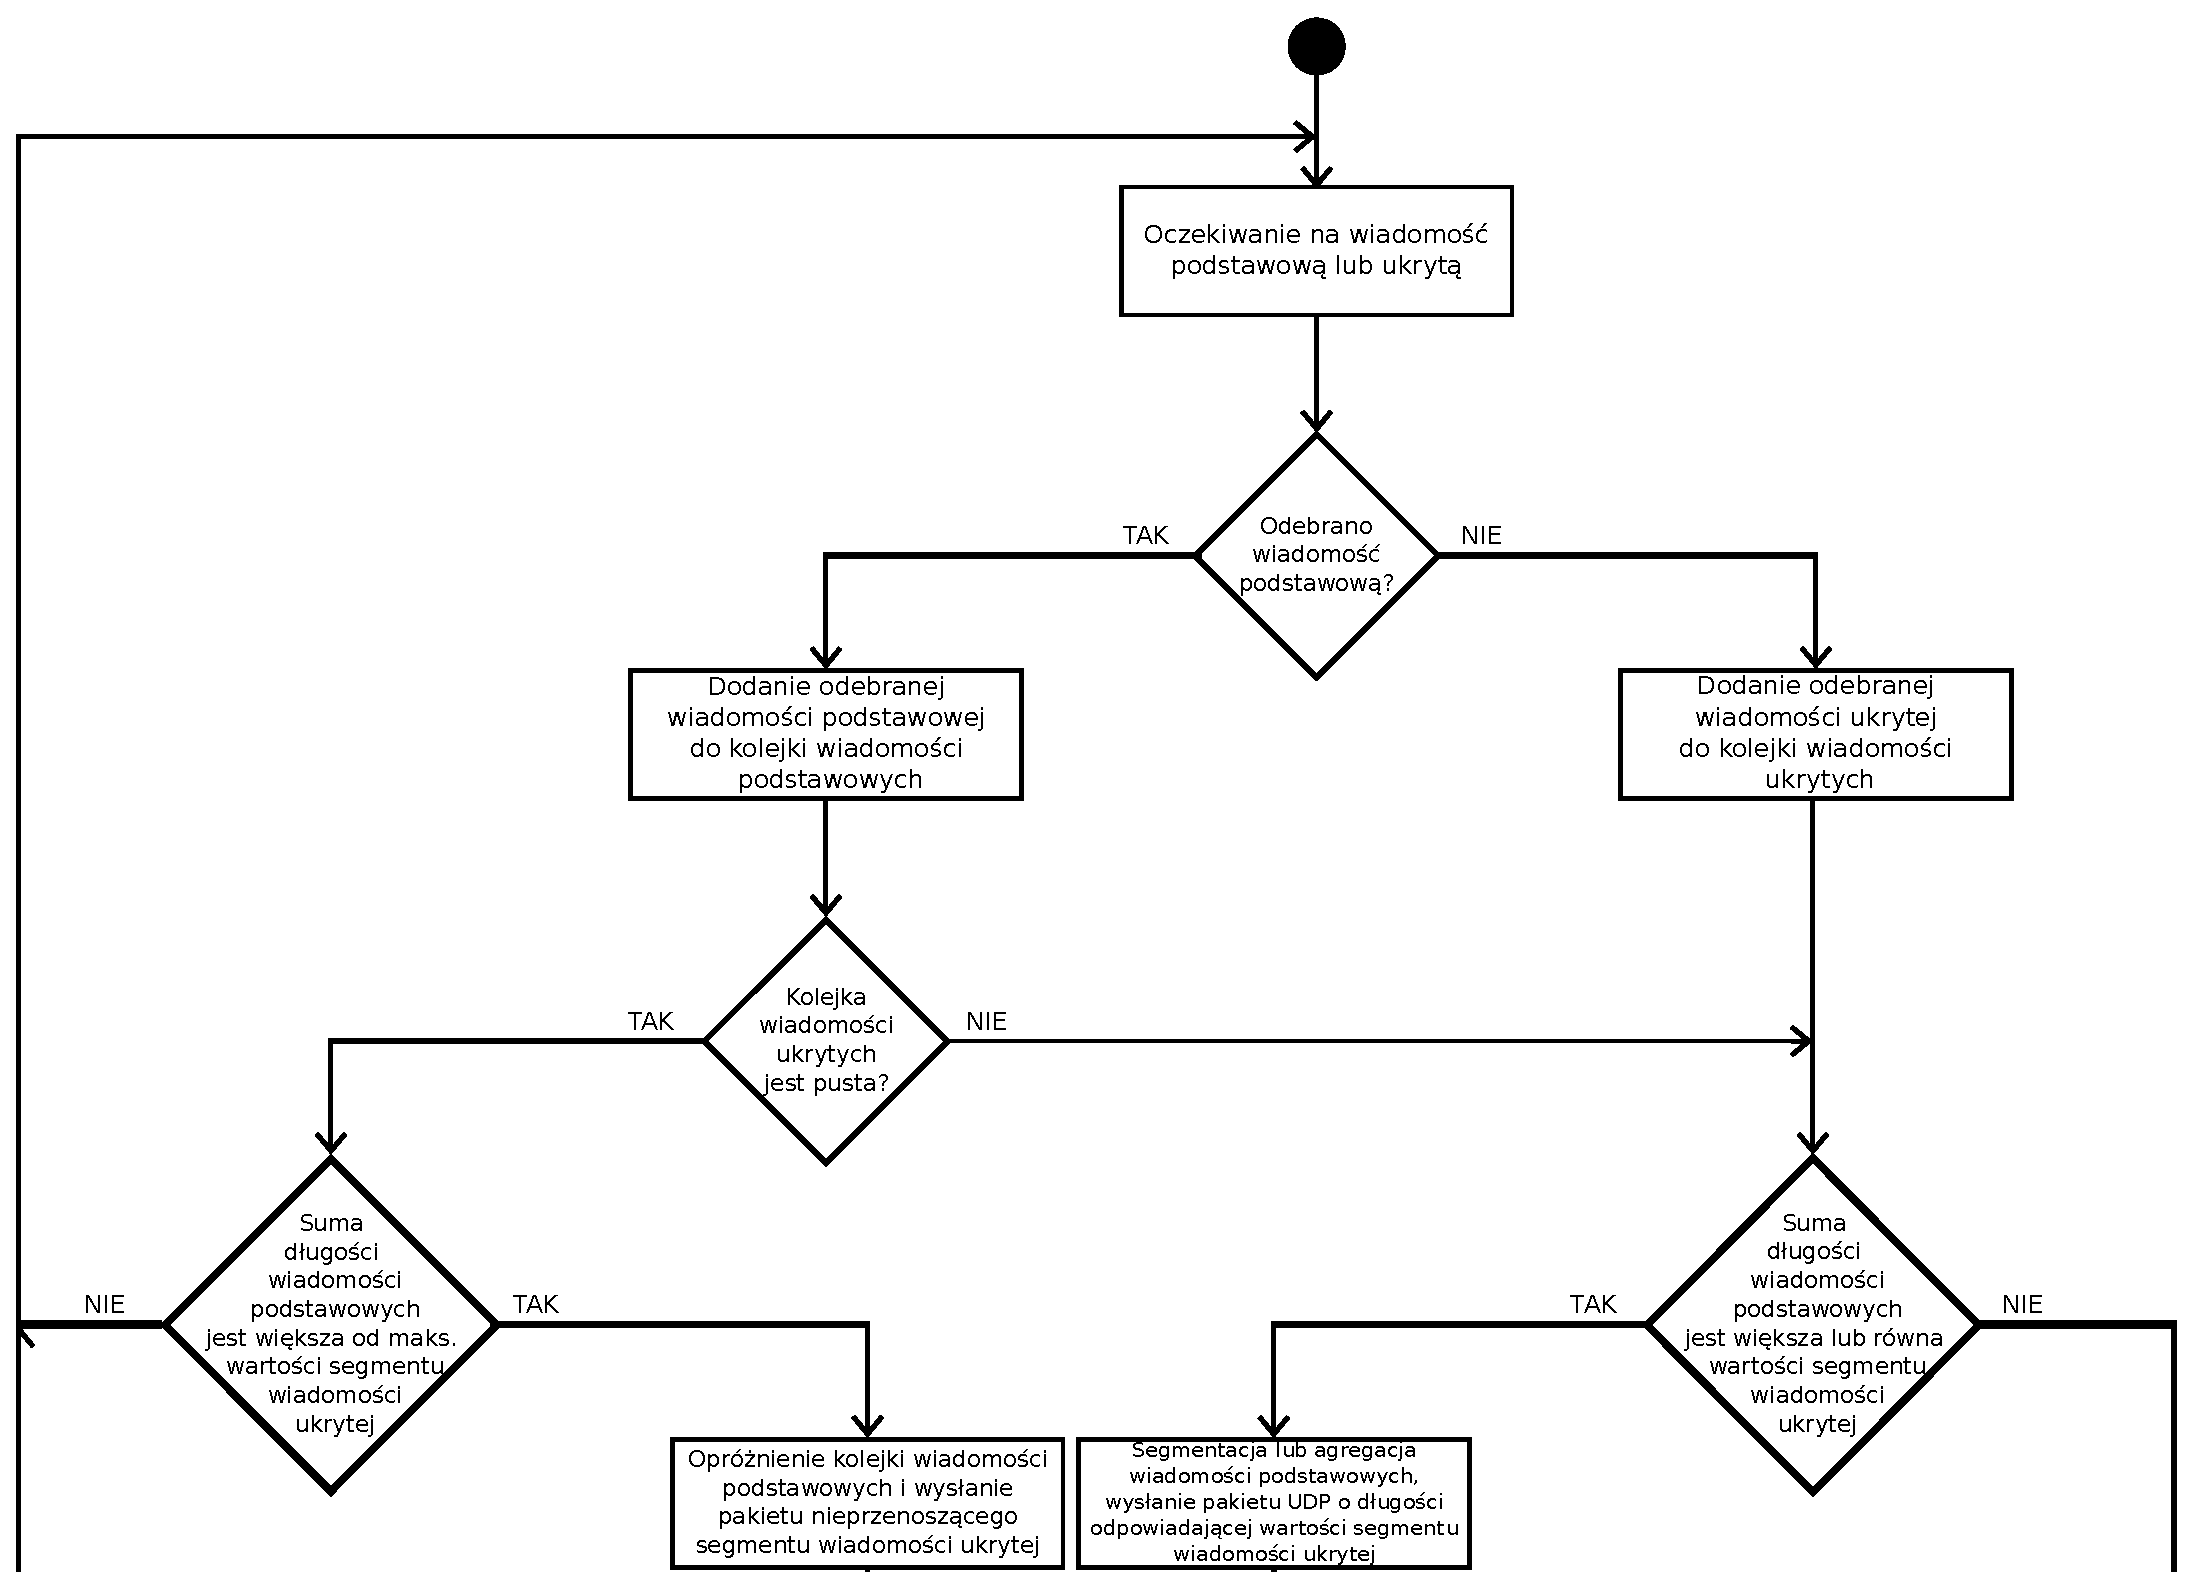
\includegraphics[scale=0.60, angle=90]{algorytm_kanalu_ukrytego}
                \caption{Schemat algorytmu kanału ukrytego}
                \label{CHANNELALGORITHM}
        \end{figure}

\chapter{Badania ilościowych charakterystyk kanału ukrytego i~kanału podstawowego dla zaproponowanego protokołu kanału ukrytego}
    \section{Wprowadzenie - zakres i~cel eksperymentów symulacyjnych}
    Zaplanowane i~omawiane w~dalszych częściach tego rozdziału eksperymenty symulacyjne,
    polegające na badaniu ilościowych zależności wybranych charakterystyk kanałów
    ukrytego i~podstawowego oraz środowiska komunikacyjnego, są uzasadnione konstrukcją
    protokołu kanału ukrytego.

    Celem eksperymentów symulacyjnych jest ilościowa weryfikacja wybranych oczekiwanych właściwości
    opracowanego protokołu kanału ukrytego, w~tym:
    \begin{itemize} \itemsep1pt \parskip0pt \parsep0pt
        \item wpływu różnic intensywności źródeł wiadomości podstawowych i~ukrytych na
            efektywność transferu wiadomości ukrytych;
        \item wpływu różnic intensywności źródeł wiadomości podstawowych i~ukrytych na
            efektywność transferu wiadomości podstawowych;
        \item wpływu różnic długości wiadomości podstawowych i~ukrytych na efektywność
            transferu wiadomości podstawowych;
        \item wrażliwości protokołu kanału podstawowego na zaproponowany protokół
            kanału ukrytego;
    \end{itemize}

    Oznaczenia:
    \begin{itemize} \itemsep1pt \parskip0pt \parsep0pt
        \item \( R_{WU} \) - średnia intensywność napływu wiadomości ukrytych (parametr rozkładu Poissona);
        \item \( L_{WU} \) - średnia długość wiadomości ukrytej (liczba segmentów - parametr rozkładu Poissona);
        \item \( V_{SWU} \) - średnia wartość segmentu wiadomości ukrytej;
        \item \( R_{WP} \) - średnia intensywność napływu wiadomości podstawowych (parametr rozkładu Poissona);
        \item \( L_{WP} \) - średnia długość wiadomości podstawowej (liczba bajtów - parametr rozkładu Poissona);
        \item \( C_P \) - pojemność kanału podstawowego (w bajtach na sekundę);
        \item \( D_{WU} \) - średnie opóźnienie wiadomości ukrytych;
        \item \( D_{WP} \) - średnie opóźnienie wiadomości podstawowych;
        \item \( L_{SWU} \) - długość segmentu danych ukrytych (parametr kanału ukrytego, w bitach);
    \end{itemize}



    \section{Zależność średniego opóźnienia wiadomości ukrytych od intensywności napływu wiadomości podstawowych}
        \subsection{Cel badania}
            Celem eksperymentu było zbadanie zależności średniego opóźnienia wiadomości (wskaźnik jakości - \( D_{WU} \))
            ukrytych od intensywności napływu wiadomości podstawowych (zmienna - parametr - \(R_{WP}\)).
            Badania zostały przeprowadzone dla różnych średnich wartości długości wiadomości
            podstawowych. \\
            Badana zależność: \\
                $$ D_{WU} = f(R_{WP} | L_{WP}, L_{SWU}, C_P, V_{SWU}, L_{WU}, R_{WU}) $$
            gdzie:\\
                \( D_{WU} \) - średnie opóźnienie wiadomości ukrytych w funkcji zmiennej \( R_{WP}, R_{WP} \in [0;5]\) \\
                dla ustalonych: \\
                \( R_{WU}  = 4 \) [wiadomość / sekundę]  \\
                \( L_{WU}  = 1 \) [ segment / wiadomość ]\\
                \( V_{SWU}  = 100 \)\\
                \( C_P  = 1000 \) [ bajty / sekundę ]\\
                \( L_{SWU}  = 16 \) [ bity ]\\
                \( L_{WP}  \in \left\{50, 100, 150\right\} \)[ bajt ] \\
        \subsection{Przebieg badania i~wnioski}
            Wartości parametrów symulacji zostały dobrane w~taki sposób, aby dane podstawowe
            były wykorzystywane głównie do transmisji danych ukrytych, co osiągnięto
            dzięki wysokiej wartości parametru ,,długość segmentu wiadomości ukrytej''.
            Badanie polegało na symulacji działania protokołu ukrytego przez okres czasu
            \( T = 5000 \). Po zakończeniu symulacji, zostało obliczone
            średnie opóźnienie wiadomości ukrytych.
            Symulacja została powtórzona \( 100 \) razy, a~wyniki z~poszczególnych
            symulacji uśredniono i~pokazano na wykresie \ref{OPOZNIENIEUKRYTYCHODPODSTAWOWYCH}

            Segment wiadomości ukrytej nie może zostać wysłany, dopóki suma długości
            wiadomości w~kolejce wiadomości podstawowych nie będzie wystarczająca do jego wysłania.
            W przeciwnym przypadku wiadomość ukryta oczekuje w~kolejce wiadomości
            ukrytych, a~jej opóźnienie rośnie. Z badań wynika, że gdy intensywność
            napływu wiadomości podstawowych jest znacznie mniejsza od intensywności
            napływu wiadomości ukrytych, średnie opóźnienie wiadomości ukrytych jest
            bardzo duże. W~takim przypadku, mała zmiana intensywności napływu wiadomości
            podstawowych ma duży wpływ na opóźnienie wiadomości ukrytych. Badania
            pokazały, że również długość wiadomości podstawowych ma wpływ na to opóźnienie.
            Intensywność i średnia długość wiadomości mogą być stosowane zamiennie
            w zadaniach zapewnienia zakładanego średniego opóźnienia wiadomości ukrytych.

            W~przypadku, gdy opóźnienie wiadomości ukrytych ma duże znaczenie,
            nie ma wielu możliwości działania. Zmniejszenie wartości parametru ,,długość
            segmentu wiadomości ukrytej'' spowoduje, że odbiorca szybciej otrzyma
            pojedyncze segmenty wiadomości, jednak ponieważ wiadomość traktujemy jako odebraną,
            po odebraniu wszystkich jej segmentów, opóźnienie całej wiadomości
            nie ulegnie zmianie.

        \begin{figure}[h]
                \centering
                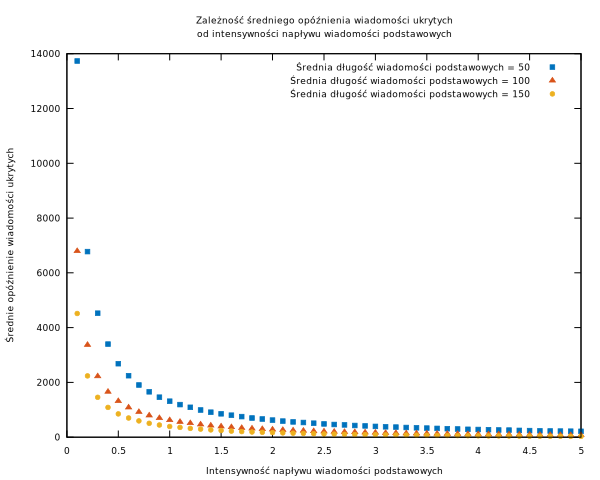
\includegraphics[]{ukrytych_od_podstawowych}
                \caption{Zależność średniego opóźnienia wiadomości ukrytych od
                    intensywności napływu wiadomości podstawowych}
                \label{OPOZNIENIEUKRYTYCHODPODSTAWOWYCH}
        \end{figure}

    \section{Zależność średniego opóźnienia wiadomości podstawowych od intensywności napływu wiadomości ukrytych} \label{OPOZNIENEPODSTAWOWYCHODUKRYTYCH}
        \subsection{Cel badania}
            Celem eksperymentu było zbadanie zależności pomiędzy intensywnością
            napływu wiadomości ukrytych (parametr - zmienna - \( R_{WU} \)), a~średnim opóźnieniem wiadomości podstawowych (wskaźnik jakości - \( D_{WP} \)).
            Badania zostały przeprowadzone dla różnych średnich długości wiadomości
            podstawowych oraz intensywności ich napływu, co pozwoliło zaobserwować
            zróżnicowane zachowanie kanału ukrytego w~zależności od wartości tych
            parametrów

            Badana zależność: \\
                $$ D_{WP} = f(R_{WU} | L_{WP}, L_{SWU}, C_P, V_{SWU}, L_{WU}, R_{WU}) $$
            gdzie:\\
                    \( D_{WP} \) - średnie opóźnienie wiadomości podstawowych w funkcji zmiennej \( R_{WU}, R_{WU} \in [0;10] \) \\
           dla ustalonych: \\
                    \( L_{WU} = 1 \) [ segment / wiadomość ]\\
                    \( V_{SWU} = 100 \)\\
                    \( C_P = 1000 \) [ bajty / sekundę ]\\
                    \( L_{SWU} = 12 \) [ bity ]\\
                    \( R_{WP} \in \left\{ 1, 5, 9 \right\}\) [ wiadomość / sekundę ]\\
                    \( L_{WP} \in \left\{ 30, 100, 400 \right\}\) [ bajt ]\\
        \subsection{Przebieg badania i~wnioski}
            Zakres zmienności wybranych wartości parametru ,,średnia długość
            wiadomości podstawowej - \(  L_{WP} \)'' w~stosunku do wartości parametru
            ,,średnia wartość segmentu wiadomości ukrytej - \( V_{SWU} \)'',
            spowodował wystąpienie trzech sposobów postępowania z wiadomościami podstawowymi
            opisanych w sekcji \ref{CHANNELDESCRIPTION}:
        \begin{itemize}
            \item konieczność agregacji kilku wiadomości podstawowych w~celu transmisji pakietu z danymi ukrytymi,
            \item dopasowanie długości wiadomości podstawowych do wartości segmentów wiadomości ukrytych,
            \item konieczność fragmentacji wiadomości podstawowych, których długość wystarcza do transmisji kilku segmentów wiadomości ukrytych.
        \end{itemize}
            Występowanie wszystkich trzech wariantów przekłada
            się na zróżnicowanie krzywych otrzymanych podczas badania zależności.

            Aby wytłumaczyć zaobserwowane zależności, zostanie wprowadzone równanie
            mówiące o~równowadze napływu wiadomości ukrytych i~napływu wiadomości podstawowych:
            \begin{equation} \label{ROWNANIEROWNOWAGI}
            R_{WP} * L_{WP} = R_{WU} * L_{WU} * V_{SWU}
            \end{equation}
            Gdy:
            \begin{itemize}
                \item obie strony równania są sobie w~przybliżeniu równe, nie ma konieczności
            kolejkowania wiadomości podstawowych ani ukrytych;
                \item lewa strona jest
            większa od prawej (w sensie średnim), oznacza to, że suma długości napływających wiadomości podstawowych
            jest większa, od wymaganej do transmisji napływających segmentów wiadomości ukrytych,
            a tym samym długość kolejki wiadomości podstawowych może rosnąć, powodując
            wzrost średniego opóźnienia wiadomości podstawowych. Dla ograniczenia tak
            wnoszonych opóźnień niezbędne jest na przykład okresowe opróżnianie kolejki
            wiadomości podstawowych poprzez wysyłanie pakietów UDP bez ich modyfikacji
            zawartością wiadomości ukrytych;
                \item prawa strona jest
            większa od lewej (w sensie średnim), oznacza to, że suma długości napływających wiadomości
            podstawowych jest niewystarczająca do transmisji wszystkich napływających
            segmentów wiadomości ukrytych, w~związku z czym rośnie długość kolejki
            segmentów wiadomości ukrytych
    \end{itemize}

            Wiadomość podstawowa może być wysłana na dwa sposoby:
            \begin{enumerate}
                \item w~pakiecie z danymi ukrytymi - sytuacja, gdy w~kolejce
                    segmentów wiadomości ukrytych znajduje się segment, do transmisji którego
                    wiadomość podstawowa może być wykorzystana, sposób ten wymaga
                    napływu wiadomości ukrytych;
                \item w~pakiecie bez segmentu wiadomości ukrytej - sytuacja, gdy suma długości wiadomości
                    podstawowych w kolejce jest większa od
                    maksymalnej wartość segmentu wiadomości ukrytej i kolejka segmentów wiadomości
                    ukrytych jest pusta. Wszystkie wiadomości w kolejce wiadomości
                    podstawowych są agregowane i wysyłane w jednym pakiecie UDP;
            \end{enumerate}

            Dzięki drugiemu sposobowi, otrzymane krzywe są ograniczone od góry.
            Ma on kluczowe znaczenie, gdy lewa strona równania \ref{ROWNANIEROWNOWAGI} jest większa od prawej.
            W~takim przypadku
            opóźnienie wiadomości podstawowych zależy od czasu zgłoszenia ostatniej
            wiadomości podstawowej, której nadejście powoduje, że suma długości oczekujących
            wiadomości podstawowych jest większa od wartości maksymalnej segmentu wiadomości ukrytej.
            Opóźnienie to jest tym mniejsze im większe jest natężenie napływu wiadomości
            i~im większa jest średnia długość napływających wiadomości. Jest to widoczne na wykresie
            \ref{OPOZNIENIEPODSTAWOWYCHODUKRYTYCH} (na przykład żółta krzywa zaczyna
            się niżej niż pomarańczowa).

            Wraz ze wzrostem intensywności napływu wiadomości ukrytych - dla danych:
            średniej intensywności napływu i średniej długości wiadomości podstawowych, wzrasta udział
            pierwszego sposobu sposobu obsługi strumienia wiadomości podstawowych.
            Oznacza to, że stopniowo zmniejsza się średnie opóźnienie wiadomości podstawowych,
            spadek ten znacznie przyspiesza, gdy obie strony równania zaczynają się wyrównywać.
            Po wyrównaniu się stron równania \ref{ROWNANIEROWNOWAGI},
            opóźnienie wiadomości podstawowych stabilizuje się, a~dalsze zwiększanie
            intensywności napływu wiadomości ukrytych nie zmniejsza go.

        \begin{figure}[h]
                \centering
                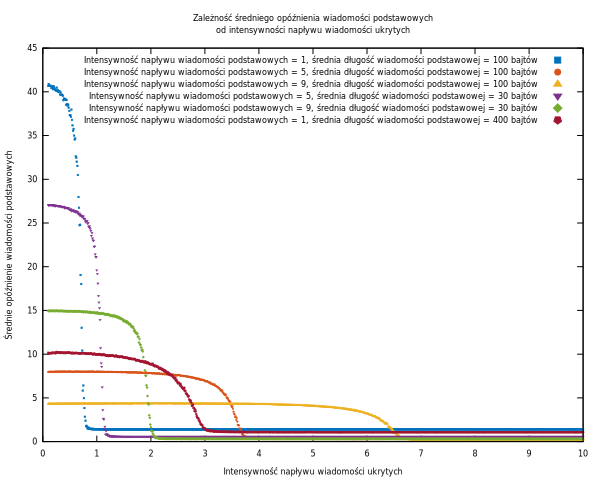
\includegraphics{podstawowych_od_ukrytych}
                \caption{Zależność średniego opóźnienia wiadomości podstawowych od
                    intensywności napływu wiadomości ukrytych}
                \label{OPOZNIENIEPODSTAWOWYCHODUKRYTYCH}
        \end{figure}



    \section{Zależność średniego opóźnienia wiadomości podstawowych od natężenia napływu wiadomości podstawowych} \label{BADANIEDLUGOSCISEGMENTUDANYCHUKRYTYCH}
        \subsection{Cel badania}
            Suma długości wiadomości podstawowych wymagana do wysłania pakietu UDP
            bez segmentu wiadomości ukrytej,
            zależy od maksymalnej wartości segmentu wiadomości ukrytej, która
            z kolei zależy od parametru konfiguracyjnego kanału ukrytego -- ,,długość segmentu wiadomości ukrytej''.
            Celem eksperymentu było zbadanie wpływu tego parametru (oznaczenie \(L_{SWU}\))
            na średnie opóźnienie wiadomości podstawowych (oznaczenie \( D_{WP} \))
            wtedy, gdy intensywność napływu wiadomości ukrytych (oznaczenie \( R_{WP} \)) jest względnie mała.
            \\
            Badana zależność: \\
                $$ D_{WP} = f(R_{WP} | L_{WP}, R_{WP}, L_{SWU}, C_P, V_{SWU}, L_{WU}) $$
            gdzie: \\
                \( D_{WP} \) - średnie opóźnienie wiadomości podstawowych, w funkcji zmiennej \( R_{WP}, R_{WP} \in [0;10] \)
           dla ustalonych: \\
                \( R_{WU} = 0.5 \) [ wiadomość / sekundę ]\\
                \( L_{WU} = 1 \) [ segment / wiadomość ]\\
                \( V_{SWU} = 5 \)\\
                \( C_P = 1000 \) [ bajty / sekundę ]\\
                \( L_{SWU} \in \left\{4, 8, 10\right\}\) [ bity ]\\
                \( L_{WP} = 5 \) [ bajt ]\\
        \subsection{Przebieg badań i~wnioski}
            Wartości parametrów symulacji zostały dobrane tak, aby system obsługi
            wprowadzał duże średnie opóźnienie wiadomości podstawowych. Mała wartość intensywności
            napływu wiadomości ukrytych (w porównaniu z intensywnością napływu wiadomości podstawowych),
            mała liczba segmentów w~pojedynczej
            wiadomości ukrytej oraz mała wartość średnia segmentu
            wiadomości ukrytej (prawa strona równania \ref{ROWNANIEROWNOWAGI} jest mniejsza od lewej strony)
            powodują, że wiadomości podstawowe są kolejkowane i
            w~konsekwencji -- są transmitowane głównie w~pakietach bez danych ukrytych.

            Jeżeli intensywność napływu wiadomości podstawowych
            jest niższa niż intensywność napływu wiadomości ukrytych (lewa część wykresu),
            to średnie opóźnienie wiadomości
            podstawowych jest małe, ponieważ szybkość obsługi wiadomości podstawowych jest
            determinowana szybkością obsługi wiadomości ukrytych (wszystkie wiadomości podstawowe transmitowane
            są w~pakietach UDP po modyfikacji przez segment wiadomości ukrytych).

            Jeżeli intensywność napływu wiadomości
            podstawowych jest większa niż intensywność napływu wiadomości ukrytych, są one kolejkowane,
            co powoduje zwiększenie wartości średniego opóźnienia wiadomości podstawowych.
            Liczba wiadomości podstawowych niezbędna do transmisji wiadomości ukrytej
            zależy od długości wiadomości ukrytych (w segmentach),
            przez co średnia liczba wiadomości podstawowych, które opuszczają kolejkę wiadomości
            podstawowych w~jednostce czasu nie jest stała. Powoduje to, że pomimo,
            że wiadomości podstawowe napływają intensywniej niż wiadomości ukryte,
            niektóre z wiadomości podstawowych, które normalnie musiałyby zostać
            wysłane w~pakiecie bez danych ukrytych, zostają wysłane w~pakietach
            z~danymi ukrytymi, w~związku z czym kolejka wiadomości podstawowych
            ulega opróżnieniu. Im większa jest wartość intensywności napływu wiadomości
            podstawowych, przy ustalonej intensywności napływu wiadomości ukrytych,
            tym rzadziej wyżej opisana sytuacja ma miejsce, co powoduje
            wzrost średniego opóźnienia wiadomości podstawowych, aż do wartości
            maksymalnej, ograniczonej przez proces wysyłania pakietów bez segmentu wiadomości ukrytej.

            Dalszy wzrost intensywności napływu wiadomości podstawowych, przy danej
            intensywności napływu wiadomości ukrytych, powoduje
            spadek średniego ich opóźnienia. Związane jest to z tym, że im intensywniej
            napływają wiadomości podstawowe, dla założonej intensywności napływu wiadomości
            ukrytych, tym mniej czasu jest potrzebne na skompletowanie sumy długości
            wiadomości podstawowych większej od wartości maksymalnej segmentu, to znaczy
            do wysłania pakietu UDP nieprzenoszącym segmentu wiadomości ukrytej.

            Przeprowadzone badania pokazują, że im mniejsza jest wartość parametru
            kanału ukrytego -- ,,długość segmentu danych ukrytych'' -- tym mniejsze
            jest maksymalne średnie opóźnienie wiadomości podstawowych, niezależnie
            od intensywności ich napływu. Warto zwrócić uwagę, że przy skrajnie małej wartości tego
            parametru, średnie opóźnienie wiadomości podstawowych w coraz mniejszym stopniu
            zależy od intensywności napływu wiadomości podstawowych. Dzieje się tak, ponieważ długość praktycznie
            każdej wiadomości podstawowej jest większa większa od maksymalnej wartości
            segmentu wiadomości ukrytej, w~związku z tym, jeśli
            kolejka segmentów wiadomości ukrytych jest pusta, wiadomość podstawowa jest
            bezzwłocznie wysłana w~pakiecie UDP nie zawierającym danych ukrytych.

        \begin{figure}[h]
                \centering
                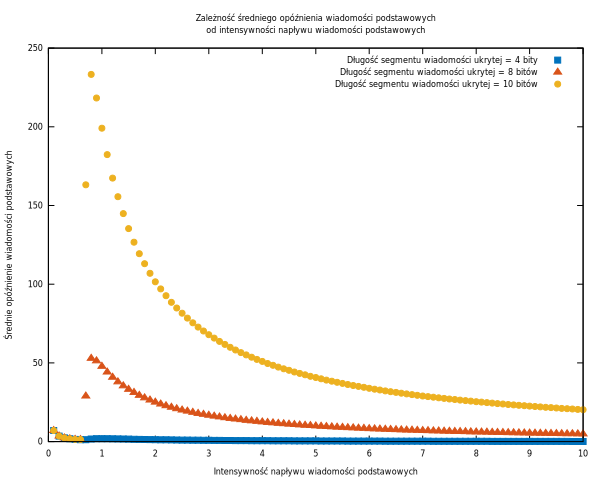
\includegraphics{podstawowych_od_podstawowych}
                \caption{Zależność średniego opóźnienia wiadomości podstawowych od
                    intensywności napływu wiadomości podstawowych}
                \label{OPOZNIENIEPODSTAWOWYCHODPODSTAWOWYCH}
        \end{figure}

        \section{Podsumowanie}
        Przeprowadzone badania pomogły poznać niektóre z~cech charakterystycznych
        proponowanego protokołu kanału ukrytego, jednak zakres przeprowadzonych badań
        jest daleki od wyczerpujących. Zbadane
        zostały zaledwie podstawowe zależności, a jedyną miarą jakości obsługi,
        mierzoną podczas eksperymentów było opóźnienie.

        Badania mogą zostać rozszerzone na dwa sposoby:
        \begin{enumerate}
            \item badanie zależności opóźnienia od wartości pozostałych parametrów źródeł
                danych, środowiska oraz kanału ukrytego, wymienionych w rozdziale;
            \item zbadanie zależności innych miar jakości obsługi od wartości parametrów
                źródeł danych, środowiska oraz kanału ukrytego, przykładem miary
                wartej zbadania, jest zmienność opóźnienia wiadomości zarówno
                podstawowych jak i ukrytych;
            \end{enumerate}

\chapter{Analiza wykrywalności kanału ukrytego}
    \section{Analiza ingerencji kanału ukrytego w~kanał podstawowy}
        Przedstawiony protokół kanału ukrytego silnie wpływa na, i~zmienia
        wartości parametrów strumienia wiadomości podstawowych. Właściwości każdego pakietu wygenerowanego
        w~kanale podstawowym są modyfikowane przez algorytm protokołu kanału ukrytego,
        czy to poprzez przechowywanie wiadomości podstawowych w~kolejce, w~celu
        ich agregacji, czy też
        poprzez ich fragmentację w~celu dostosowania długości transmitowanej wiadomości
        do wartości segmentu wiadomości ukrytej. Duża ingerencja w kanał podstawowy
        została podyktowana chęcią uzyskania kompromisu pomiędzy przepływnością
        kanału ukrytego (zwiększoną dzięki kolejkowaniu wiadomości podstawowych),
        a~jego wykrywalnością (zmniejszoną, dzięki zastosowaniu pakietów nieprzenoszących danych ukrytych,
        zmniejszającymi maksymalne opóźnienie wiadomości podstawowych).
        W przypadku (statystycznie pomijalnym) gdy długość wiadomości podstawowej
        jest równa wartości oczekującego segmentu danych ukrytych, wiadomość podstawowa
        jest transmitowana bezzwłocznie (pod warunkiem, że przepływność kanału podstawowego
        jest większa od intensywności źródła wiadomości podstawowych). W takich przypadkach
        wiadomość podstawowa nie jest zmieniana i sposób obsługi nie wnosi dodatkowego
        opóźnienia. W ogólnym przypadku, zaproponowany sposób obsługi segmentów wiadomości
        ukrytych zmienia charakterystyki strumienia wiadomości podstawowych.
        Sposób oddziaływania kanału ukrytego na strumień wiadomości podstawowych
        może być podstawą do konstruowania ataków na protokół kanału ukrytego,
        a~w~związku z tym, zasadne jest rozważenie możliwości wyboru takich wartości
        parametrów kanału ukrytego ukrytego, które zwiększają poziom bezpieczeństwa
        komunikacji. Bezpieczeństwo komunikacji zależy od prawdopodobieństwa
        wykrycia faktu transmisji wiadomości ukrytych, które jest tym większe,
        im bardziej zmienione zostaną parametry strumienia wiadomości podstawowych.

        Z badania przedstawionego w~sekcji \ref{OPOZNIENEPODSTAWOWYCHODUKRYTYCH},
        wynika, że największe średnie opóźnienia wiadomości podstawowych
        występuje wtedy, gdy zarówno natężenie napływu wiadomości podstawowych, jak i~ukrytych, jest małe.
        Jeśli ponadto natężenie napływu wiadomości ukrytych jest mniejsze niż wiadomości podstawowych,
        powoduje to, że wiadomości podstawowe są agregowane.
        W~takiej sytuacji niewielka liczba wiadomości podstawowych jest w~stanie
        opuścić kolejkę w pakiecie zawierającym dane ukryte, a~czas potrzebny do
        zagregowania wystarczającej ilości danych do zbudowania pakietu nie
        zawierającego danych ukrytych jest duży. W~skrócie można powiedzieć, że
        im mniejsze jest natężenie napływu wiadomości ukrytych w~stosunku do natężenia
        napływu wiadomości podstawowych, tym większe jest średnie opóźnienie wiadomości podstawowych.
        Jak pokazano w~sekcji \ref{BADANIEDLUGOSCISEGMENTUDANYCHUKRYTYCH},
        średnie opóźnienie wiadomości podstawowych można do pewnego stopnia ograniczyć, odpowiednio
        dobierając wartość długość segmentu wiadomości ukrytej - parametr protokołu
        kanału ukrytego.

        Z idei działania przedstawionego protokołu kanału ukrytego, wynika, że wpływa on na strumień
        wiadomości podstawowych, poprzez zmianę długości pakietów UDP, którymi są one transmitowane.
        Zaproponowany protokół kanału ukrytego, nie daje dużych możliwości konfiguracji i~wpływu
        na długość nadawanych pakietów, a~minimalizacja tego rodzaju ingerencji
        w~zaproponowanym protokole jest trudna. Pozwala to atakującemu
        na wykorzystanie analizy statystycznej i~porównawczej, w~celu detekcji
        wykorzystania kanału ukrytego.

    \section{Metody ataku na protokół kanału ukrytego}
       W~tej sekcji zostaną przedstawione metody ataku na zaproponowany protokół kanału ukrytego. Omówione
       zostaną zarówno techniki będące w~arsenale steganoanalizy aktywnej jak i
       pasywnej. Rozważane są metody wykorzystujące wiedzę na temat metody organizacji kanału ukrytego
       i~sposobów jego ingerencji w~strumień wiadomości podstawowych, które zostały
       przedstawione w~poprzedniej sekcji, jak również metody ślepe (\emph{ang. blind}).

       \subsection{Detekcja kanału ukrytego}
       W~sieciach komputerowych, w~których bezpieczeństwo ma duże znaczenie często
       stosowane są systemy IDS (\emph{and. Intrusion detection system}). Tego typu
       systemy opierają się na regułach opisujących ruch sieciowy występujący w
       sieci w~czasie normalnego funkcjonowania. Reguły te mogą być wprowadzone ręcznie
       przez człowieka, lub wywnioskowane przez system za pomocą rejestracji ruchu i~metod z dziedziny
       analizy statystycznej, lub rozpoznawania wzorców (jedna z gałęzi machine learning)\cite{IDSDESCRIPTION}.
       System IDS nieustannie monitoruje ruch aktualnie występujący w~sieci i~sprawdza
       jego zgodność, z określonymi wcześniej regułami. Wykrycie anomalii, lub odstępstwa
       od reguł, powoduje zgłoszenie alarmu administratorowi sieci. Użycie tego
       typu systemu jest możliwe przeciwko proponowanemu protokołowi kanału ukrytego.
       Taki system mógłby wykryć zarówno opóźnienia jak i~modyfikacje długości
       pakietów w~kanale podstawowym wprowadzone przez protokół kanału ukrytego.
       Ograniczeniem zastosowania tego typu systemów w~wykrywaniu przedstawianego kanału
       ukrytego, jest zapotrzebowanie na zasoby. W~przypadku steganoanalizy ślepej
       konieczne jest analizowanie każdego pakietu transmitowanego w~sieci. Posiadanie
       informacji o~zastosowany kanale ukrytym, pozwala na ograniczenie analizy jedynie
       do pakietów UDP, których nadal może być dużo.

       \subsection{Zakłócanie i uniemożliwianie komunikacji w~kanale ukrytym}
       Przeciwko proponowanemu protokołowi kanału ukrytego można zastosować aktywny atak steganograficzny
       oparty na ponownej fragmentacji pakietów zmodyfikowanych przez protokół
       kanału ukrytego i~transmitowanych kanałem podstawowym. Celem takiego aktywnego
       ataku jest modyfikowanie lub usuwanie ukrytych wiadomości. Pomimo, że według
       specyfikacji RFC protokół UDP jest protokołem datagramowym i~obierany przez
       odbiorcę pakiet jest dokładnie taki sam, został wysłany przez
       nadawcę, to jeśli atakujący wie, w~jak można podzielić lub zagregować
       pakiety protokołu kanału podstawowego, w~taki sposób, aby nie wpłynęło to na
       jego funkcjonowanie, może zastosować tego typu atak. Zmiana rozmiaru pakietu
       powoduje, że odbiorca interpretuje jego długość jako błędny fragment danych
       ukrytych w~stosunku do tego, który nadał nadawca. Powoduje to, że komunikacja
       kanałem ukrytym staje się utrudniona, lub nawet niemożliwa, i~atakujący osiąga
       swój cel. Na rysunku \ref{UDANYATAKAKTYWNY} przedstawiono udany atak tego typu,
       gdzie atakującemu (Ewa), poprzez agregację dwóch pakietów,
       udaje się zablokować komunikację pomiędzy Alicją i~Bobem.
        \begin{figure}[h]
                \centering
                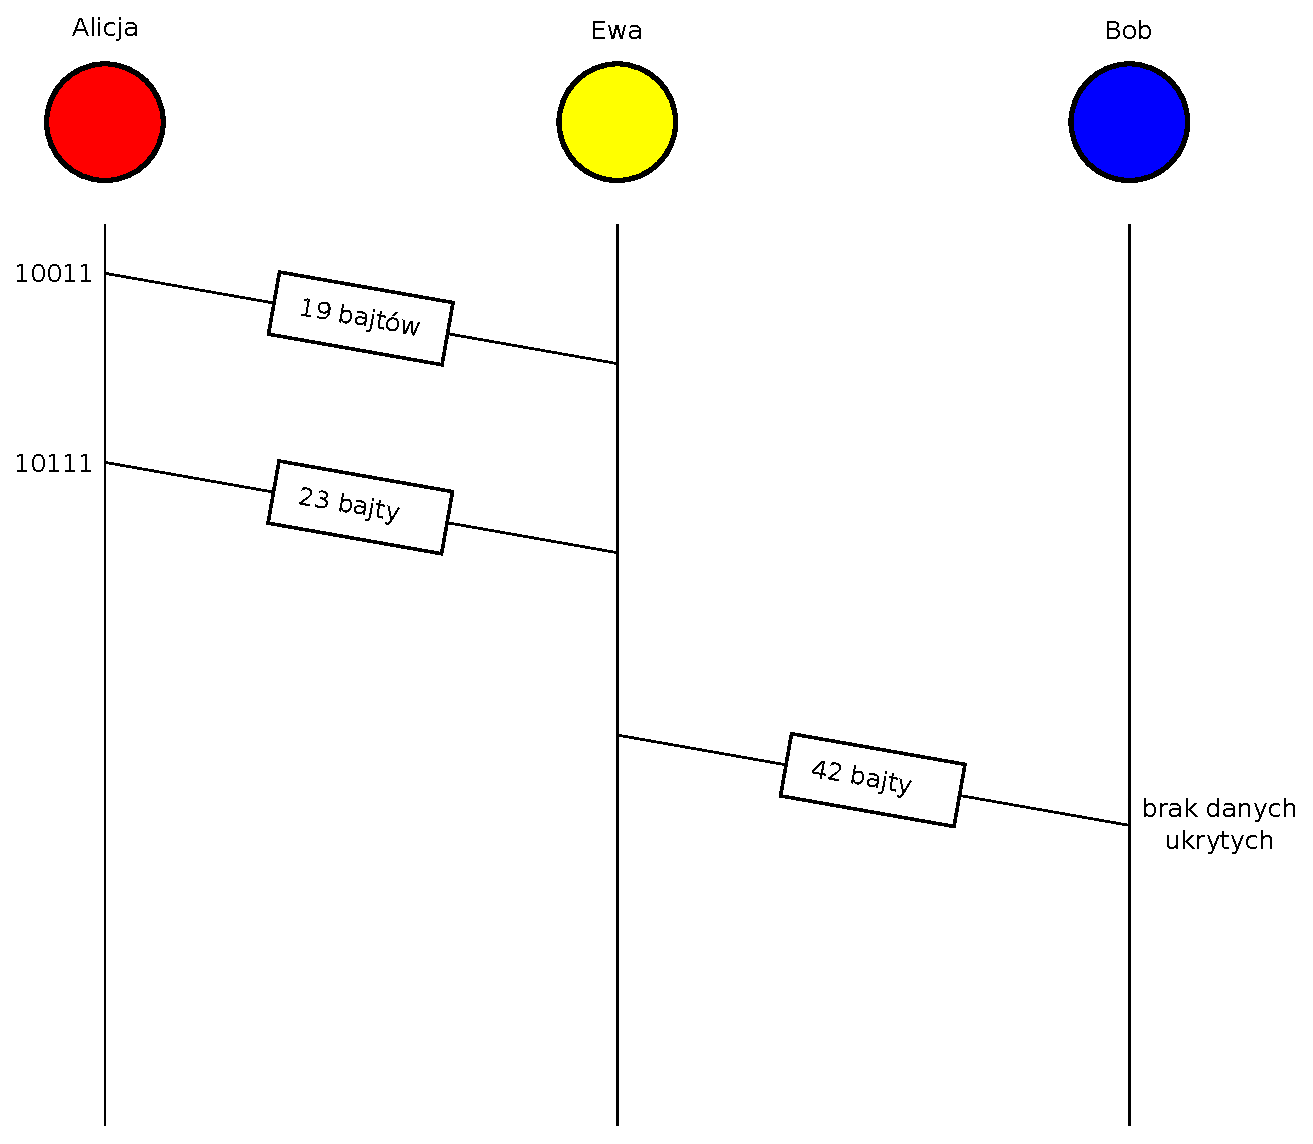
\includegraphics[scale=0.7]{udany_atak}
                \caption{Udany atak aktywny na protokół kanału ukrytego}
                \label{UDANYATAKAKTYWNY}
        \end{figure}
       Należy zauważyć, że dzięki braku obsługi błędów w~kanale ukrytym
       i~braku jego reakcji w~odpowiedzi na błędy w~trakcie transmisji danych, atakujący
       nie dostaje żadnej informacji zwrotnej mówiącej, czy atak się powiódł. Gdyby
       poprzez taki atak, zostałaby wykonana na przykład retransmisja błędnie odebranej
       wiadomości, byłby to ewidentny dowód na to, że ukryty kanał jest wykorzystywany.
       W~tym kontekście brak obsługi błędów przez kanał ukryty można traktować więc
       jako zaletę.

       \subsection{Odczytywanie wiadomości ukrytych}
       Po wykryciu komunikacji w kanale ukrytym, atakujący może chcieć
       odczytać treść segmentów wiadomości ukrytych. Protokół kanału ukrytego posiada
       jeden parametr - długość segmentu wiadomości ukrytej, który
       może być traktowany jako klucz algorytmu, ponieważ zgodnie z definicją podaną
       w~sekcji \ref{STEGANOGRAFIAPOJECIA}, dla tego samego nośnika i~takiej samej
       wiadomości ukrytej, w~zależności od wartości tego parametru generowane są
       inne steganogramy (pakiety UDP o~różnych długościach). Wartość tego parametru wpływa również
       na interpretację długości pola danych pakietów UDP przez odbiorcę danych ukrytych.
       Na przykład pakiety o~długościach odpowiednio 4 i~12 bajtów, dla \( L_{SWU} = 4 \)
       zostaną zinterpretowane jako \( 0100 \) \( 1100 \), natomiast dla \( L_{SWU} = 5 \)
       jako \( 00100 \) \( 01100 \), co pokazuje, że aby odczytać zawartość wiadomości
       ukrytych, atakujący musi poznać wartość klucza użytego w~algorytmie protokołu
       kanału ukrytego.

       Zbiór wartości tego
       klucza jest z góry ograniczony przez specyfikację protokołu UDP, w którym
       definiowana jest maksymalna długość datagramu (16 bitowe pole).
       Wynika z tego maksymalna długość pakietu UDP: \(2^{16} - 1 = 65535\) bajtów. Jest to również maksymalna
       wartość segmentu wiadomości ukrytej, jaki może być transmitowany pojedynczym
       pakietem zawierającym dane ukryte. Wynika z tego, że istnieje jedynie 16
       dozwolonych wartości klucza: \( L_{SWU} \in N \land L_{SWU} \in [1, 16] \),
       co pozwala na zastosowanie ataku siłowego w~celu złamania klucza.

       W~dziedzinie zapewniania bezpieczeństwa komunikacji, ustalanie wartości
       klucza od zawsze stanowiło duży problem. W~tym celu zostały opracowane
       dedykowane algorytmy, na przykład algorytm Diffiego-Hellmana. Zastosowanie
       ich w~przypadku steganografii może ułatwić wykrycie kanału ukrytego. Należy tutaj przypomnieć,
       że podstawowym celem steganografii jest ukrycie faktu istnienie ukrytej wiadomości.
       Wykorzystaniu wcześniej wspomnianych algorytmów wymiany kluczy towarzyszy
       wymiana charakterystycznych dla tych algorytmów pakietów danych. W~przypadku
       wykrycia tego typu pakietów przez podsłuchującego może się on domyślić,
       że istnieje jakaś ukryta wiadomość i~na przykład zablokować komunikację lub
       zastosować techniki przedstawione w~poprzedniej sekcji. Pod tym względem
       kanały ukryte nie wymagające użycia kluczy, lub wymagające prostych kluczy,
       nie wymagających skomplikowanych protokołów ich wymiany, takie jak prezentowany
       protokół kanału ukrytego, mogą prezentować
       się lepiej od protokołów używających skomplikowanych kluczy.

       Alternatywnym atakiem, jest atak z wykorzystaniem analizy statystycznej.
       Należy zauważyć, że dany segment wiadomości ukrytej, jest zawsze transmitowany
       za pomocą pakietu UDP o~takiej samej długości (zakładając ustaloną wartość klucza -
       długości segmentu wiadomości ukrytej). Powoduje to przenoszenie wzorców i
       prawidłowości występujących w~tekście wiadomości ukrytych, na ciąg długości
       pakietów UDP transmitowanych kanałem podstawowym. Jest to podatność analogiczna
       do występującej na przykład w~szyfrze Cezara. Pozwala ona na zastosowanie
       ataku statystycznego, opartego na znajomości tekstu jawnego, lub informacji
       na temat jego charakterystyk, do złamania klucza użytego w~algorytmie protokołu
       kanału ukrytego.

    \section{Sugestie doboru parametrów proponowanego kanału ukrytego} \label{SUGESTIEPARAMETROW}
       Z dotychczasowych rozważań na temat wykrywalności proponowanego kanału ukrytego, wynika,
       że głównym sposobem wykrycia jego wykorzystywania jest analiza jego ingerencji
       w~strumień wiadomości podstawowych. W~związku z tym dobór parametrów protokołu
       kanału ukrytego minimalizujących stopień
       tej ingerencji może znacznie utrudnić potencjalnemu atakującemu wykrycie
       wiadomości ukrytych.

       Podstawową i~strategiczną kwestią jest wybór protokołu warstwy aplikacji kanału podstawowego,
       z którym współpracował będzie protokół kanału ukrytego. Decyzja ta powinna zostać
       podjęta po oszacowaniu zapotrzebowania na przepływność kanału ukrytego,
       zidentyfikowaniu strumienia wiadomości ukrytych (na przykład średniej długości,
       średniego natężenia napływu wiadomości, oraz ich typowej treści).
       Celem tych oszacowań jest dobór takiego protokołu
       kanału podstawowego, który będzie miał charakterystyki (średnią długość wiadomości
       i~natężenie ich napływu) jak najbardziej zbliżone do zapotrzebowań określonych
       wcześniej. Zbliżone natężenie napływu wiadomości podstawowych i~ukrytych zapewnia,
       że wprowadzone do kanału podstawowego opóźnienia nie będą duże.
       Zbliżone długości wiadomości podstawowych do wartości segmentów wiadomości ukrytych,
       sprawiają, że nawet po fragmentacji przeprowadzonej przez algorytm kanału ukrytego,
       wygenerowane pakiety będą miały długość zbliżoną do naturalnie występującej
       w~kanale podstawowym. Zdecydowanie odradzane jest wykorzystanie protokołów
       charakteryzujących się krótkimi wiadomościami i~małą intensywnością ich napływu,
       w~badaniach zostało pokazane, że powodują one powstawanie dużych opóźnień.
       Protokoły generujące duże ilości wiadomości sprawdzają się w~większości
       przypadków (na przykład VoIP, protokoły transmisji strumieniowej).
       Inną istotną cechą dobrego protokołu kanału podstawowego jest duża różnorodność
       długości napływających wiadomości, co zapewnia, że IDS nie podniesie alarmu,
       gdy protokół kanału ukrytego będzie generował pakiety o~różnej długości,
       w~zależności od danych ukrytych.

       Problem małego natężenia napływu wiadomości ukrytych można rozwiązać poprzez
       odpowiedni dobór wartości parametru długość segmentu wiadomości ukrytej.
       Niska jego wartość powoduje, że agregacja ilości danych niezbędnych do
       wysłania pakietu bez danych ukrytych trwa krócej, co w~konsekwencji zmniejsza
       opóźnienie wprowadzane do kanału podstawowego. Zmniejszenie wartości tego parametru powoduje generowanie
       krótszych pakietów, co zwiększa narzut ze strony nagłówka pakietu. W~małych
       pakietach stosunek długości nagłówka pakietu do długości danych jest niekorzystny.
       Powoduje to, że aby uniknąć opóźnień wymagana jest większa pojemność kanału
       podstawowego.

    \section{Inne sposoby obrony przed wykryciem}
       Poza wyborem kanału podstawowego i~konfiguracją protokołu kanału ukrytego,
       w~celu utrudnienia wykrycia transmisji ukrytych wiadomości i~zwiększenia
       bezpieczeństwa transmisji można także:
       \begin{itemize}
           \item Skompresować dane ukryte przed transmisją - dzięki zastosowaniu
               kompresji, wysłanie danych ukrytych wymaga mniejszej ilości
               danych podstawowych. Może to pozwolić na użycie kanału ukrytego
               w~warunkach, gdzie natężenie napływu wiadomości podstawowych
               jest niewystarczające. Ponadto kompresja pozwala usunąć z treści
               wiadomości charakterystyczne dla niej, powtarzające się wzorce,
               co pozwala zmniejszyć zagrożenie ze strony analizy statystycznej
               prowadzonej w~celu złamania klucza algorytmu steganograficznego.
               Kompresja powoduje także, że charakterystyka treści wiadomości nie jest widoczna
               w~ciągu długości pakietów generowanych przez protokół kanału ukrytego.
           \item Dodatkowo wykorzystać kryptografię - zaszyfrowanie danych, pozwala
               zabezpieczyć treść wiadomości ukrytej, przed próbą jej odczytania w
               przypadku odkrycia jej istnienia. Może jednak spowodować wspomniane
               wcześniej problemy z ustaleniem klucza kryptograficznego przed rozpoczęciem
               komunikacji. Nowoczesne algorytmy szyfrujące charakteryzują się
               tym, że kryptogramy przez nie stworzone, nie zawierają żadnych wzorców,
               mają charakterystykę zbliżoną do szumu, co wpływa na długości pakietów
               generowanych przez kanał ukryty podobnie jak kompresja.
           \item Wykorzystać wiele kanałów ukrytych - jeśli w~sieci komputerowej
               wykorzystywane jest wiele protokołów opartych o~protokół transportowy UDP,
               możliwe jest stworzenie wielu kanałów ukrytych, z których każdy dedykowany
               byłby transmisji innych wiadomości. Na przykład kanał oparty o~protokół
               DNS (generujący dużo małych wiadomości)  mógłby być wykorzystywany
               do transmisji stosunkowo krótkich, ale nie cierpiących zwłoki wiadomości
               ukrytych, natomiast kanał oparty o~protokół TFTP (protokół transferu plików,
               generujący duże wiadomości, jednak uruchamiany stosunkowo rzadko)
               byłby używany do transmisji większych wiadomości ukrytych. Dzięki
               temu długości wiadomości ukrytych są bardziej dopasowane do charakterystyk
               wiadomości podstawowych, co zmniejsza potrzebę znacznej ingerencji
               w~ich rozmiar.

           \item Zastosowanie długości segmentu wiadomości ukrytej, nie będącego
               dzielnikiem długości słowa maszynowego - jeśli wiadomość ukryta
               zawiera jakiś wzorzec, powtarzające się fragmenty, najczęściej fragmenty
               te mają długość równą, lub będącą wielokrotnością długości słowa maszynowego.
               Związane jest to z tym, że komputery najszybciej działają na danych
               o~właśnie takiej długości, w~związku z tym w~takiej postaci są one przesyłane
               przez sieć. Zastosowanie długości segmentu wiadomości ukrytej nie będącej
               dzielnikiem długości powtarzającego się fragmentu, powoduje, że generowanych
               jest mniej segmentów o~takich samych wartościach, a~w konsekwencji,
               mniej pakietów o~takich samych długościach. Jak pokazano na rysunku \ref{REPETEDFRAGMENTS}
               segmenty o~takich samych wartościach zaczynają się powtarzać po
               przetworzeniu liczby bitów będącej najmniejszą wspólną wielokrotnością
               długości powtarzającego się fragmentu i~przyjętej długości segmentu
               (40 bitów dla segmentu o~długości 5 bitów i~8 bitów dla segmentu o
               długości 4 bitów).

                \begin{figure}[h]
                        \centering
                        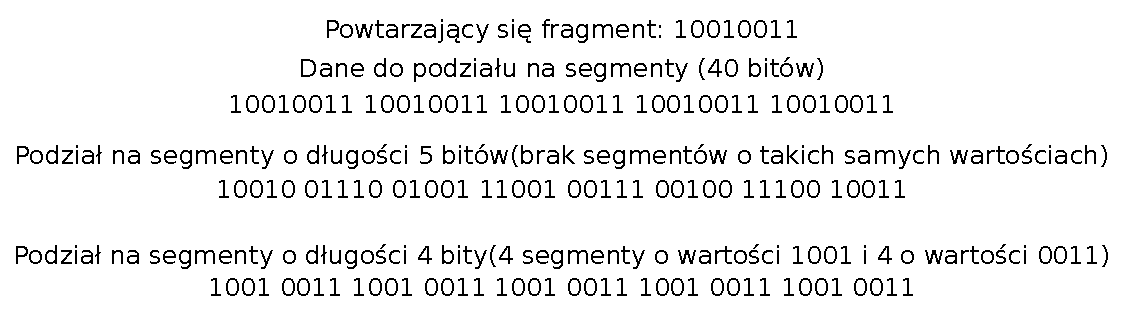
\includegraphics[scale=0.75]{powtorzone_fragmenty}
                        \caption{Wpływ długości segmentu na ilość segmentów o~takich samych wartościach}
                        \label{REPETEDFRAGMENTS}
                \end{figure}
       \end{itemize}


\chapter{Podsumowanie i~wnioski}
    W~pracy przedstawiony został protokół sieciowego kanału ukrytego,
    opartego o~interpretację długości pakietów protokołu UDP, jako wartości fragmentów
    danych ukrytych. Przeprowadzone zostały badania zależności wartości wybranego
    wskaźnika jakości komunikacji (średnie opóźnienie wiadomości) od wartości wybranych
    parametrów charakteryzujących strumienie wiadomości podstawowych i~wiadomości ukrytych
    oraz protokół kanału ukrytego.  Na podstawie tych badań, przedstawiono ogólne
    uwagi dotyczące wykrywalności zaproponowanego kanału ukrytego oraz przedstawione
    zostały sugestie mające na celu ograniczenie wykrywalności.

    W oparciu o  przeprowadzone analizy, stwierdzono, że prezentowany protokół
    kanału ukrytego, mógłby być zastosowany w~realnym systemie sieci komputerowej.
    Dzięki odpowiedniej konfiguracji, doborowi odpowiedniego protokołu kanału
    podstawowego oraz zastosowaniu przedstawionych wskazówek,
    wykrywalność ukrytego kanału można utrzymać na akceptowalnym
    poziomie, dla typowych zastosowań cywilnych.

    Do zalet przedstawionego kanału ukrytego należy zaliczyć:
    \begin{itemize}
        \item Prostotę działania - zasada działania protokołu kanału ukrytego
            nie jest skomplikowana, co przekłada się na łatwość i~niski koszt
            ewentualnej implementacji takiego protokołu. Umożliwia ona także
            dokładną analizę kanału i~dostosowanie go do konkretnego środowiska,
            oraz ułatwia jego potencjalną rozbudowę.
        \item Dużą dostępność protokołów mogących służyć jako kanał podstawowy -
            jedynym wymaganiem stawianym protokołowi kanału podstawowego jest
            wykorzystanie jako protokołu transportowego protokołu UDP. Dzięki temu
            zbiór takich protokołów jest duży, co umożliwia zastosowanie kanału
            ukrytego w~różnorodnych środowiskach sieciowych.
        \item Możliwość komunikacji z użyciem węzłów pośredniczących - z uwagi
            na datagramową naturę protokołu UDP, węzły pośredniczące nie mogą stosować
            agregacji, ani fragmentacji pakietów w~celu optymalizacji ich transmisji.
            Wobec tego, długość nadanego pakietu nie zmienia się w~czasie transmisji
            z udziałem pośrednika, i~dociera on do odbiorcy dokładnie w~takiej postaci
            jak został nadany przez nadawcę.
        \item Przepływność i~niskie opóźnienia w~ kanale ukrytym - dzięki
            zastosowaniu kolejkowania i~agregacji wiadomości podstawowych,
            czas oczekiwania na agregację wystarczającej liczby wiadomości podstawowych do zbudowania
            pakietu zawierającego segment danych ukrytych jest mniejszy, niż na przykład
            w~przypadku, gdy segment wiadomości ukrytej musiałby oczekiwać na
            wiadomość podstawą o~dokładnie takiej samej długości jak wartość segmentu.
        \item Brak wrażliwości na błędy podstawieniowe - ze względu na to, że jako
            fragment danych ukrytych interpretowana jest długość pakietu UDP, protokół
            kanału ukrytego nie zwraca uwagi na zawartość tych pakietów.
            Błędy podstawieniowe powodują zmianę treści wiadomości a~nie ich długości, na skutek tego,
            nie powodują one błędu w~transmisji segmentu danych ukrytych. Protokół
            nie jest jednak wrażliwy na zagubienie bitów pakietu, lub ich wtrącenie.
    \end{itemize}

    Natomiast jako wady kanału ukrytego można wymienić:
    \begin{itemize}
        \item Podatność na atak siłowy - mała liczebność zbioru możliwych do zastosowania
            kluczy steganograficznych powoduje, że może być on łatwo złamany,
            przy użyciu najprostszego ataku steganograficznego, polegającego
            na przeglądzie jego wszystkich możliwych wartości.
        \item Konieczność dostosowania konfiguracji kanału do środowiska - protokół
            kanału ukrytego nie dostarcza domyślnych wartości parametrów konfiguracyjnych, a
            uzyskanie satysfakcjonujących parametrów jego działania, wymaga dostosowania
            parametrów konfiguracyjnych do konkretnego środowiska sieciowego,
            w~którym ma on być wykorzystywany.
        \item Znaczną ingerencję w~kanał podstawowy - jak zostało wspomniane wcześniej,
            każda wiadomość podstawowa jest kolejkowana, bądź fragmentowana przez
            protokół kanału ukrytego, co przy nieodpowiedniej konfiguracji może
            przełożyć się na znaczną zmianę parametrów działania kanału podstawowego.
        \item Przenoszenie charakterystyk wiadomości ukrytych na długości generowanych pakietów UDP -
            przekazywanie powtarzających się segmentów danych ukrytych
            zawsze pakietem o~takiej samej długości, powoduje wyciek informacji
            statystycznych na temat treści wiadomości ukrytych. Sprawia to, że
            kanał ukryty jest podatny na, co prawda bardziej skomplikowany od ataku siłowego,
            ale również prosty, atak statystyczny.

    \end{itemize}
\chapter{Możliwości rozwoju i~kontynuacji prac}
    Pomimo przeprowadzenie badań zależności miar jakości usługi od wartości wybranych
    parametrów źródeł ruchu i wartości parametrów protokołu kanału ukrytego,
    oraz przeprowadzenia analizy wykrywalności przedstawianego kanału ukrytego, nadal kryje on kilka tajemnic.

    Podstawową kwestią jest prawdziwa implementacja protokołu kanału ukrytego
    i~jego uruchomienie w~realnym środowisku sieciowym. Pozwoliłoby to przeprowadzić
    te same badania na "żywym organizmie" i~sprawdzić osiągane parametry w~warunkach polowych.
    Uruchomienia protokołu w~sieci komputerowej, umożliwiłoby przeprowadzenie opisanego
    wcześniej procesu dopasowania parametrów konfiguracyjnych protokołu do konkretnego
    środowiska sieciowego i~praktyczne sprawdzenie skuteczności oraz wpływu takich
    działań na wykrywalność kanału ukrytego. Ponadto, możliwe byłoby uruchomienie
    kanału ukrytego w~sieciach komputerowych, w~których wykorzystywany jest system
    detekcji intruzów (IDS) i~praktyczną ocena tego, jak dobrze tego typu systemy
    radzą sobie z detekcją wykorzystania kanału ukrytego, oraz co można zrobić,
    aby im to utrudnić. Analiza uruchomionej w~sieci implementacji kanału ukrytego,
    na pewno pozwoliłaby na wyciągnięcie dużej ilości propozycji na udoskonalenie
    protokołu kanału ukrytego.

    Na podstawie przeprowadzonych w~symulatorze badań, oraz analizy wykrywalności
    kanału ukrytego, również można wysunąć propozycje dalszych prac nad kanałem ukrytym:

    \begin{itemize}
        \item Zmiana funkcji definiującej rozmiar pakietu UDP dla pojedynczego segmentu danych ukrytych -
            jednym z głównych problemów protokołu kanału ukrytego, jest wyciek
            informacji statystycznych na temat wiadomości ukrytych.
            Większe zaawansowanie rozważanej funkcji, mogłoby ograniczyć ten problem.
            Można tu przytoczyć mechanizm analogiczny do zastosowanego w~szyfrze
            homofonicznym, dzięki któremu jednemu segmentowi danych ukrytych
            odpowiadałoby kilka możliwych długości pakietów UDP, a~wspomniana funkcja
            wybierałaby jeden z nich na przykład losowo, lub przy pomocy algorytmu
            karuzelowego.
        \item Przesyłanie niektórych wiadomości podstawowych w~postaci niezmienionej -
            kolejny poważny problem kanału ukrytego polega na dużej ingerencji w
            strumień wiadomości podstawowych. Ingerencja ta może zostać ograniczona, poprzez
            transmisję niektórych wiadomości z kanału podstawowego, natychmiast
            po ich napłynięciu, bez kolejkowania, w~niezmienionej postaci.
            Pozwala to na większe zachowanie oryginalnych charakterystyk kanału
            podstawowego. Takie pakiety nie przenoszą danych ukrytych, w~związku
            z czym konieczna jest sygnalizacja tego faktu odbiorcy, na przykład
            z wykorzystaniem zarezerwowanego pola nagłówka.
    \end{itemize}

\clearpage
\addcontentsline{toc}{chapter}{Bibliografia}
\bibliographystyle{plain}
\bibliography{bibliografia}


\end{document}
